\documentclass[../../main/main.tex]{subfiles}
\graphicspath{{./figures/}}

\dominitoc
\faketableofcontents

% \renewcommand{\mtcSfont}{\small\bfseries}
% \renewcommand{\mtcSSfont}{\footnotesize}
\mtcsettitle{minitoc}{}
\mtcsetrules{*}{off}

\makeatletter
\renewcommand{\@chapapp}{Ondes -- chapitre}
\renewcommand{\chaplett}{ON}
\makeatother

% \toggletrue{student}
% \toggletrue{corrige}
% \renewcommand{\mycol}{black}
% \renewcommand{\mycol}{gray}

\hfuzz=5.002pt

\begin{document}
\setcounter{chapter}{1}

\settype{book}
\settype{prof}
\settype{stud}

\chapter{Interférences à deux ondes}

\vspace*{\fill}

\begin{tcn}(appl)<ctc>"somm"'t'{Sommaire}
	\let\item\olditem
	\vspace{-15pt}
	\minitoc
	\vspace{-25pt}
\end{tcn}

\begin{tcn}[sidebyside]
	(appl)<ctb>"how"'t'{Capacités exigibles}
	\begin{itemize}[label=\rcheck]
		\item Interférences entre deux ondes acoustiques, mécaniques ou lumineuses
		      de même fréquence.
		\item Différence de chemin optique. Conditions d'interférences
		      constructives ou destructives.
		\item Exemple du dispositif des trous d'\textsc{Young} éclairé par une source
		      monochromatique.
		\item Exprimer les conditions d'interférences constructives ou
		      destructives.
	\end{itemize}
	\tcblower
	\begin{itemize}[label=\rcheck]
		\item Déterminer l'amplitude de l'onde résultante en un point en fonction
		      du déphasage.
		\item Relier le déphasage entre les deux ondes à la différence de chemin
		      optique.
		\item Établir l'expression littérale de la différence de chemin optique
		      entre les deux ondes.
		\item Exploiter la formule de \textsc{Fresnel} fournie pour décrire la
		      répartition d'intensité lumineuse.
	\end{itemize}
\end{tcn}

\vspace*{\fill}
\newpage
\vspace*{\fill}

%\vspace{-15pt}
\begin{tcn}[%
		sidebyside, fontupper=\small, fontlower=\small
	](appl)<ctb>"chek"'t'{L'essentiel}
	\begin{tcn}[nsp](defi)<ctc>'t'{Définitions}
		\vspace{-25pt}
		\tcblistof[\subsubsection*]{defi}{\hspace*{4.8pt}}
	\end{tcn}
	% \begin{tcn}[nsp](rapp)<ctc>'t'{Rappels}
	% 	\vspace{-25pt}
	% 	\tcblistof[\subsubsection*]{rapp}{\hspace*{4.8pt}}
	% \end{tcn}
	\begin{tcn}[nsp](prop)<ctc>'t'{Propriétés}
		\vspace{-25pt}
		\tcblistof[\subsubsection*]{prop}{\hspace*{4.8pt}}
		% \tcblistof[\subsubsection*]{loi}{\hspace*{4.8pt}}
		% \tcblistof[\subsubsection*]{theo}{\hspace*{4.8pt}}
	\end{tcn}
	% \begin{tcn}[nsp](prop)<ctc>'t'{Théorèmes}
	% 	\vspace{-25pt}
	% 	% \tcblistof[\subsubsection*]{prop}{\hspace*{4.8pt}}
	% 	% \tcblistof[\subsubsection*]{loi}{\hspace*{4.8pt}}
	% 	\tcblistof[\subsubsection*]{theo}{\hspace*{4.8pt}}
	% \end{tcn}
	% \begin{tcn}[nsp](loi)<ctc>'t'{Lois}
	% 	\tcblistof[\subsubsection*]{loi}{\hspace*{4.8pt}}
	% \end{tcn}
	% \begin{tcn}[nsp](coro)<ctc>'t'{Corollaires}
	%   \tcblistof[\subsubsection*]{coro}{\hspace*{4.8pt}}
	% \end{tcn}
	% \begin{tcn}[nsp](demo)<ctc>'t'{Démonstrations}
	% 	\vspace{-25pt}
	% 	\tcblistof[\subsubsection*]{demo}{\hspace*{4.8pt}}
	% 	% \tcblistof[\subsubsection*]{prev}{\hspace*{4.8pt}}
	% \end{tcn}
	% \begin{tcn}[nsp](inte)<ctc>'t'{Interprétations}
	% 	\tcblistof[\subsubsection*]{inte}{\hspace*{4.8pt}}
	% \end{tcn}
	% \begin{tcn}[nsp](impl)<ctc>'t'{Implications}
	% 	\vspace{-25pt}
	% 	\tcblistof[\subsubsection*]{impl}{\hspace*{4.8pt}}
	% \end{tcn}
	% \begin{tcn}[nsp](tool)<ctc>'t'{Outils}
	% 	\tcblistof[\subsubsection*]{tool}{\hspace*{4.8pt}}
	% \end{tcn}
	% \begin{tcn}[nsp](nota)<ctc>'t'{Notations}
	% 	\tcblistof[\subsubsection*]{nota}{\hspace*{4.8pt}}
	% \end{tcn}
	% \begin{tcn}[nsp](appl)<ctc>'t'{Applications}
	% 	\vspace{-25pt}
	% 	\tcblistof[\subsubsection*]{appl}{\hspace*{4.8pt}}
	% \end{tcn}
	% \begin{tcn}[nsp](rema)<ctc>'t'{Remarques}
	%   \tcblistof[\subsubsection*]{rema}{\hspace*{4.8pt}}
	% \end{tcn}
	% \begin{tcn}[nsp](exem)<ctc>'t'{Exemples}
	%   \tcblistof[\subsubsection*]{exem}{\hspace*{4.8pt}}
	% \end{tcn}
	% \begin{tcn}[nsp](ror)<ctc>"hart"'t'{Points importants}
	%   \tcblistof[\subsubsection*]{ror}{\hspace*{4.8pt}}
	% \end{tcn}
	% \begin{tcn}[nsp](impo)<ctc>'t'{Erreurs communes}
	%   \tcblistof[\subsubsection*]{impo}{\hspace*{4.8pt}}
	% \end{tcn}
	\tcblower
	% \begin{tcn}[nsp](defi)<ctc>'t'{Définitions}
	%   \tcblistof[\subsubsection*]{defi}{\hspace*{4.8pt}}
	% \end{tcn}
	% \begin{tcn}[nsp](rapp)<ctc>'t'{Rappels}
	%   \tcblistof[\subsubsection*]{rapp}{\hspace*{4.8pt}}
	% \end{tcn}
	% \begin{tcn}[nsp](prop)<ctc>'t'{Propriétés}
	% \tcblistof[\subsubsection*]{prop}{\hspace*{4.8pt}}
	% \tcblistof[\subsubsection*]{loi}{\hspace*{4.8pt}}
	% \tcblistof[\subsubsection*]{theo}{\hspace*{4.8pt}}
	% \end{tcn}
	% \begin{tcn}[nsp](coro)<ctc>'t'{Corollaires}
	%   \tcblistof[\subsubsection*]{coro}{\hspace*{4.8pt}}
	% \end{tcn}
	\begin{tcn}[nsp](demo)<ctc>'t'{Démonstrations}
		\vspace{-25pt}
		\tcblistof[\subsubsection*]{demo}{\hspace*{4.8pt}}
		% \tcblistof[\subsubsection*]{prev}{\hspace*{4.8pt}}
	\end{tcn}
	% \begin{tcn}[nsp](inte)<ctc>'t'{Interprétations}
	% 	\tcblistof[\subsubsection*]{inte}{\hspace*{4.8pt}}
	% \end{tcn}
	% \begin{tcn}[nsp](impl)<ctc>'t'{Implications}
	% 	\tcblistof[\subsubsection*]{impl}{\hspace*{4.8pt}}
	% \end{tcn}
	% \begin{tcn}[nsp](tool)<ctc>'t'{Outils}
	% 	\vspace{-25pt}
	% 	\tcblistof[\subsubsection*]{tool}{\hspace*{4.8pt}}
	% \end{tcn}
	% \begin{tcn}[nsp](nota)<ctc>'t'{Notations}
	% 	\tcblistof[\subsubsection*]{nota}{\hspace*{4.8pt}}
	% \end{tcn}
	% \begin{tcn}[nsp](odgr)<ctc>'t'{Ordres de grandeur}
	% 	\tcblistof[\subsubsection*]{odgr}{\hspace*{4.8pt}}
	% \end{tcn}
	\begin{tcn}[nsp](appl)<ctc>'t'{Applications}
		\vspace{-25pt}
		\tcblistof[\subsubsection*]{appl}{\hspace*{4.8pt}}
	\end{tcn}
	% \begin{tcn}[nsp](rema)<ctc>'t'{Remarques}
	%   \tcblistof[\subsubsection*]{rema}{\hspace*{4.8pt}}
	% \end{tcn}
	\begin{tcn}[nsp](exem)<ctc>'t'{Exemples}
		\vspace{-25pt}
		\tcblistof[\subsubsection*]{exem}{\hspace*{4.8pt}}
	\end{tcn}
	\begin{tcn}[nsp](ror)<ctc>"hart"'t'{Points importants}
		\vspace{-25pt}
		\tcblistof[\subsubsection*]{ror}{\hspace*{4.8pt}}
	\end{tcn}
	% \begin{tcn}[nsp](impo)<ctc>'t'{Erreurs communes}
	% 	\vspace{-25pt}
	% 	\tcblistof[\subsubsection*]{impo}{\hspace*{4.8pt}}
	% \end{tcn}
\end{tcn}

\vspace*{\fill}

\newpage

\section{Introduction}
\subsection{Approximation par une onde plane}
Soit une source en un point S, émettant une onde sinusoïdale. En toute
généralité, et même sans atténuation, son amplitude dépend du point considéré~:
\[
	s(\vv{r},t) = A(r) \cos(\wt - \vv{k}\cdot \vv{r} + \f_0)
\]
\smallbreak
\vspace*{-10pt}
\noindent
avec $\vv{k}$ le vecteur d'onde et $\vv{r}$ le vecteur position en 3 dimensions.
En effet, l'énergie totale d'une perturbation se répartit selon l'espace
disponible. On les différencie alors selon les «~vagues~» qu'elles forment~:

\begin{tcb}[sidebyside, righthand ratio=.5](defi){Fronts d'ondes}
	Si les fronts d'ondes dessinent~:
	\begin{itemize}
		\item une \textbf{droite}, alors l'onde est \textbf{plane}~;
		\item un \textbf{cercle}, alors l'onde est \textbf{circulaire}~;
		\item une \textbf{sphère}, alors l'onde est \textbf{sphérique}.
	\end{itemize}
	\tcblower
	\begin{center}
		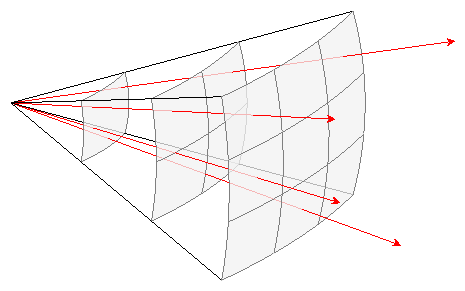
\includegraphics[width=.65\linewidth]{wave_3d_sph}
		\captionof{figure}{Front d'onde sphérique.}
	\end{center}
\end{tcb}

Pour obtenir de résultats simples, on se limite à des ondes planes avec
l'approximation suivante~:

\begin{tcb*}[sidebyside, righthand ratio=.4](prop){Approxima$^\circ$ par une onde
			plane}
	À des distances de la source S \textbf{suffisamment grandes devant la longueur
		d'onde} $\lambda$, on peut approximer la vibration $s(\Mr,t)$ par une
	\textbf{onde plane}~:
	\psw{%
		\[\boxed{s(\Mr,t) = A\cos(\wt-k\SMr +\f_0)}\]
	}%
	avec $A$ constante au voisinage de M.
	\tcblower
	\begin{center}
		\sswitch{
			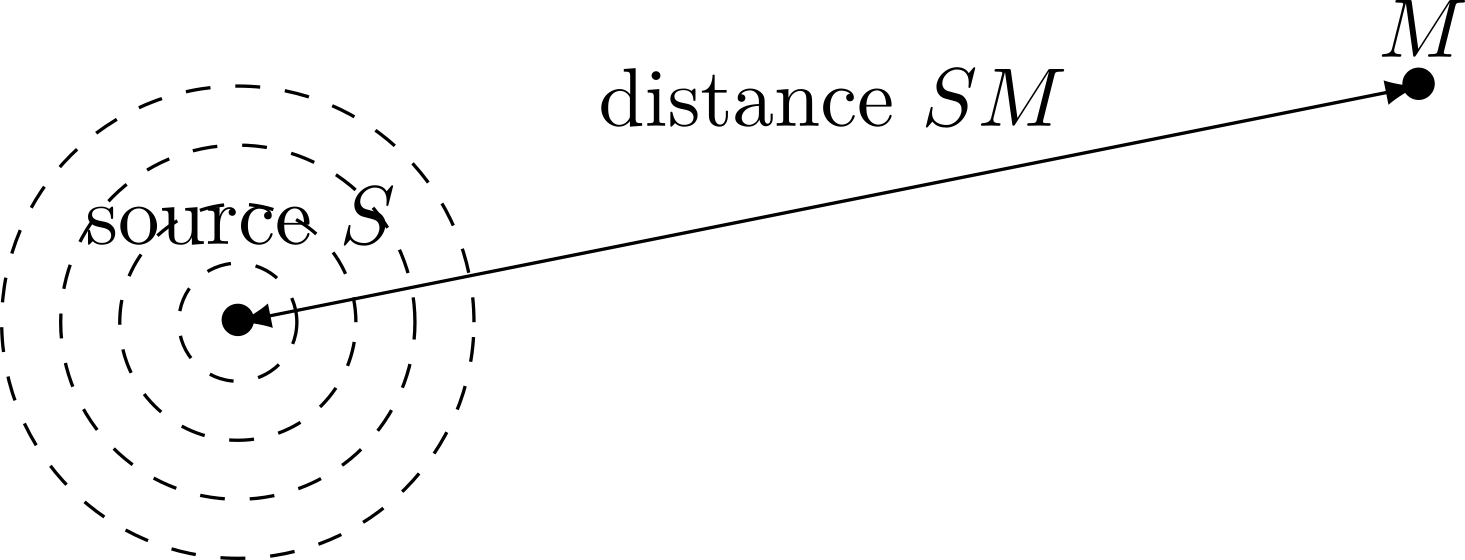
\includegraphics[width=\linewidth, draft=true]{SM}
		}{
			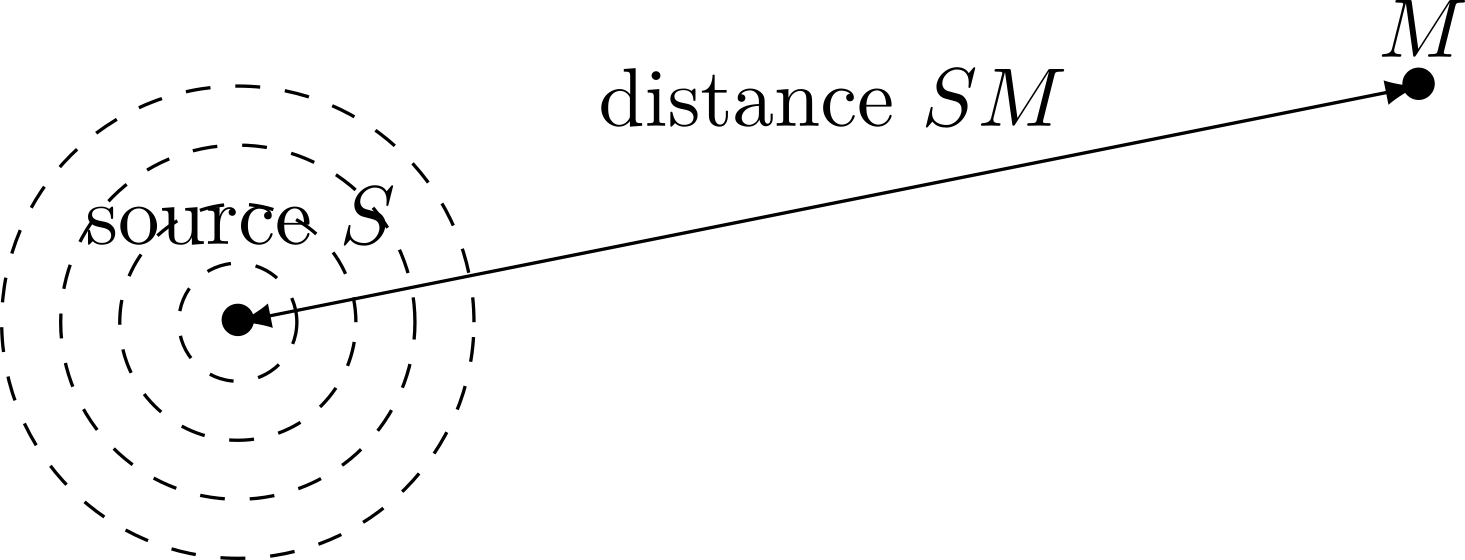
\includegraphics[width=\linewidth]{SM}
		}
		\vspace{-15pt}
		\captionsetup{justification=centering}
		\captionof{figure}{\\Approximation par une onde plane}
	\end{center}
\end{tcb*}

\subsection{Déphasage}
\begin{tcb*}[breakable](defi){Phase spatiale et déphasage}
	Soit deux signaux sinusoïdaux, de \textbf{même fréquence}, \textbf{longueur
		d'onde} et \textbf{nature}, provenant de 2 sources $\Sr_1$ et $\Sr_2$, se
	superposant en un point $\Mr$. Avec $n \in [1;2]$~:
	\smallbreak
	\begin{isd}[righthand ratio=.25]
		\vspace{-20pt}
		\psw{%
			% \begin{align*}
			%   s_1(\Mr, t) & = A_1\cos(\wt -k\SaMr + \f_{01})
			%   \\\text{et} \quad
			%   s_2(\Mr, t) & = A_2\cos(\wt -k\SbMr + \f_{02})
			% \end{align*}
			\begin{gather*}
				s_n(\Mr, t) = A_n\cos(\wt -k \mathrm{S_nM} + \f_{0n})
				% \\\text{et} \quad
				% s_2(\Mr, t) & = A_2\cos(\wt -k\SbMr + \f_{02})
			\end{gather*}
		}%
		On introduit alors pour simplifier la \textbf{phase spatiale}~:
		% \begin{align*}
		%   \f_1(\Mr) & = -k\SaMr + \f_{01}
		%   \\\text{et} \quad
		%   \f_2(\Mr) & = -k\SbMr + \f_{02}
		% \end{align*}
		\begin{gather*}
			% \f_n(\Mr) = -k\mathrm{S_nM} + \f_{0n}
			\psw{%
				\f_1(\Mr) = -k\SaMr + \f_{01}
			}%
			\qet
			\psw{%
				\f_2(\Mr) = -k\SbMr + \f_{02}
			}%
		\end{gather*}
		\vspace{-15pt}
		\tcblower
		\begin{center}
			\sswitch{
				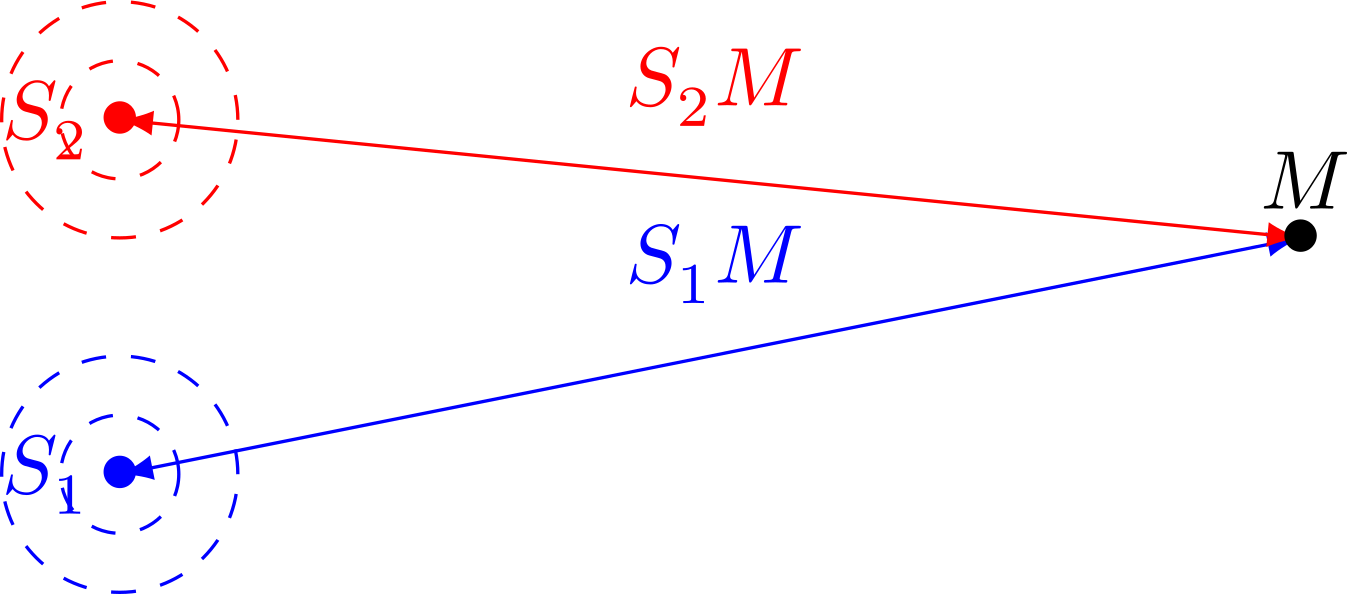
\includegraphics[width=\linewidth, draft=true]{S12M}
			}{
				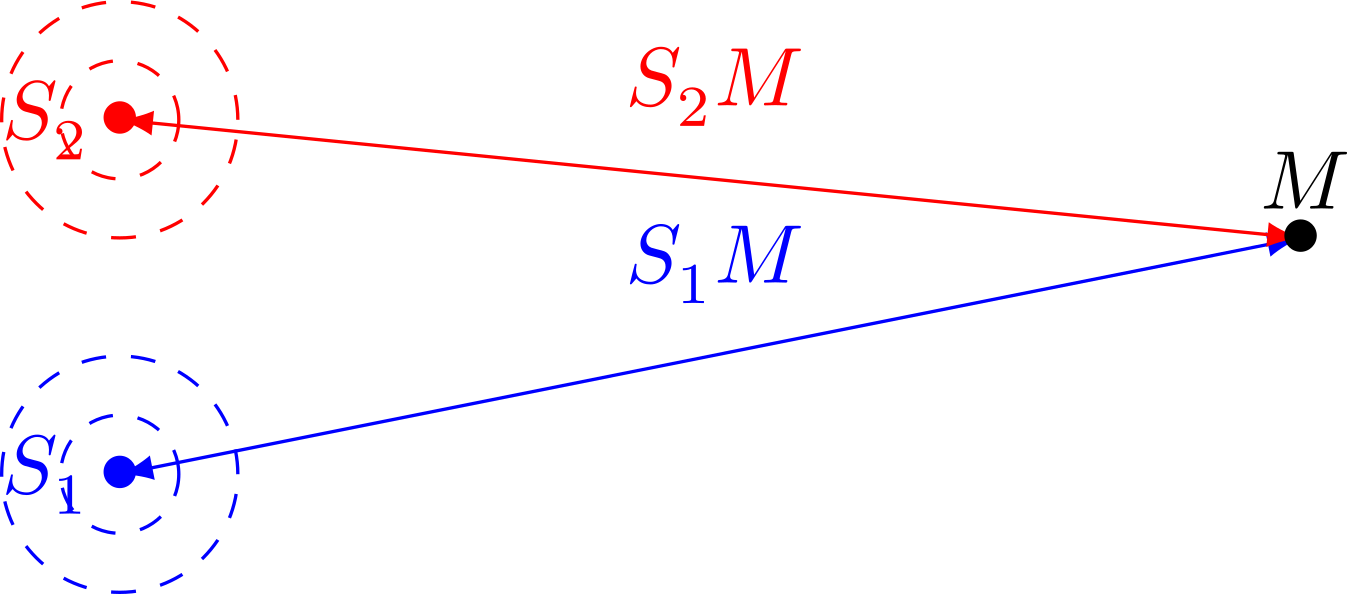
\includegraphics[width=\linewidth]{S12M}
			}
			\vspace{-15pt}
			\captionsetup{justification=centering}
			\captionof{figure}{}
		\end{center}
	\end{isd}
	Ainsi, le \textbf{déphasage} entre $s_2$ et $s_1$ se réduit à leur
	\textbf{différence de phase spatiale}~:
	\psw{%
		\[
			\D\f_{2/1}(\Mr) =
			(\wt \underbracket[1pt]{-k\SaMr + \f_{02}}_{\f_2(\Mr)}) -
			(\wt \underbracket[1pt]{-k\SbMr + \f_{01}}_{\f_1(\Mr)})
			\Lra
			\boxed{\D\f_{2/1}(\Mr) = \f_2(\Mr) - \f_1(\Mr)}
		\]
	}%
	\vspace{-15pt}
\end{tcb*}

\subsection{Valeurs particulières}
\begin{tcb}[breakable](rapp){Déphasages particuliers}
	\vspace{-10pt}
	\begin{isd}[righthand ratio=.3, interior hidden](rapp)
		\tcbsubtitle{\fatbox{\textbf{En phase}}}
		Deux signaux sont \textbf{en phase} si leur \textbf{déphasage est nul}
		(modulo $2\pi$)~:
		\[
			\D\f \equiv 0\quad[2\pi]
			\Lra
			\boxed{\D\f = 2p\pi}
			\quad p \in \Zb
		\]
		Les signaux passent par leurs valeurs maximales et minimales aux mêmes
		instants, et s'annulent simultanément.
		\tcblower
		\begin{center}
			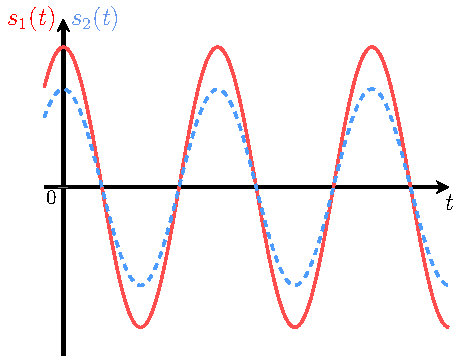
\includegraphics[width=\linewidth]{dfeq0.pdf}
			\captionsetup{justification=centering}
			\captionof{figure}{\\En phase.}
		\end{center}
	\end{isd}
	\vspace{-15pt}
	\begin{isd}[righthand ratio=.3, interior hidden](rapp)
		\tcbsubtitle{\fatbox{\textbf{En quadrature}}}
		Deux signaux sont en \textbf{quadrature phase} si leur déphasage est de
		$\mathbf{\pm\pi/2}$ (modulo $2\pi$)~:
		\[
			\D\f \equiv \pm\frac{\pi}{2} \quad[2\pi]
			\Lra
			\boxed{\D\f = \left( p+\frac{1}{2} \right)\pi}
			\quad p \in \Zb
		\]
		Quand un signal s'annule, l'autre est à son maximum où à son minimum~:
		c'est la relation entre un cosinus et un sinus.
		\tcblower
		\begin{center}
			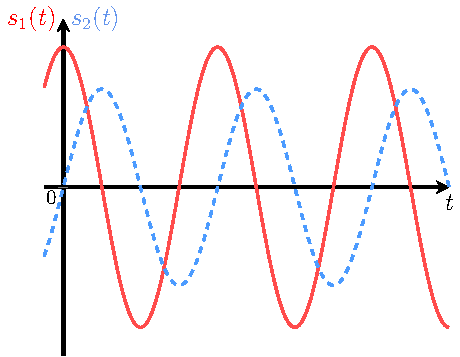
\includegraphics[width=\linewidth]{dfeqpi2.pdf}
			\captionsetup{justification=centering}
			\captionof{figure}{\\En quadrature.}
		\end{center}
	\end{isd}
	\vspace{-15pt}
	\begin{isd}[righthand ratio=.3, interior hidden](rapp)
		\tcbsubtitle{\fatbox{\textbf{En opposition}}}
		Deux signaux sont en \textbf{opposition de phase} si leur déphasage est de
		$\mathbf{\pm\pi}$ (modulo $2\pi$)~:
		\[
			\D\f \equiv \pm\pi \quad[2\pi]
			\Lra
			\boxed{\D\f = (2p+1)\pi}
			\quad p \in \Zb
		\]
		Lorsqu'un signal passe par sa valeur maximale, l'autre est à la valeur
		minimale, mais ils s'annulent simultanément.
		\tcblower
		\begin{center}
			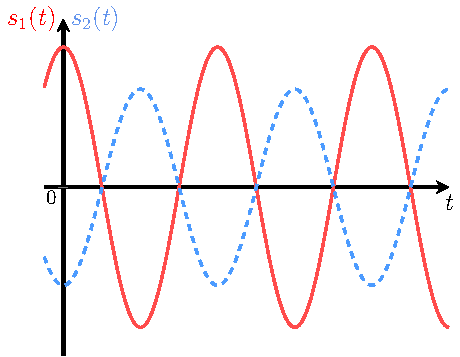
\includegraphics[width=\linewidth]{dfeqpi.pdf}
			\captionsetup{justification=centering}
			\captionof{figure}{\\En opposition.}
		\end{center}
	\end{isd}
	\vspace{-10pt}
\end{tcb}

% \subsection{Lecture d'un déphasage en représentation temporelle}
% \begin{tcb*}[sidebyside, righthand ratio=.3](prop){Lecture d'un déphasage}
% 	Le déphasage $\D\f_{2/1}$ est lié au \textbf{retard temporel}
% 	$\D{t}_{2/1} = t_2 - t_1$ du signal $s_2$ par rapport au signal $s_1$~: on a
% 	\psw{%
% 		\[\boxed{\abs{\D\f_{2/1}} = \pm \w \abs{\D{t}_{2/1}}}\]
% 	}%
% 	Le déphasage obtenu est entre $-\pi$ et $+\pi$. On définit~:
% 	\begin{itemize}
% 		\item \psw{%
% 			      $\D\f_{2/1} > 0 \Rightarrow s_2$ est en avance sur $s_1$~;
% 		      }%
% 		\item \psw{%
% 			      $\D\f_{2/1} < 0 \Rightarrow s_2$ est en retard sur $s_1$.
% 		      }%
% 	\end{itemize}
% 	\tcblower
% 	\begin{center}
% 		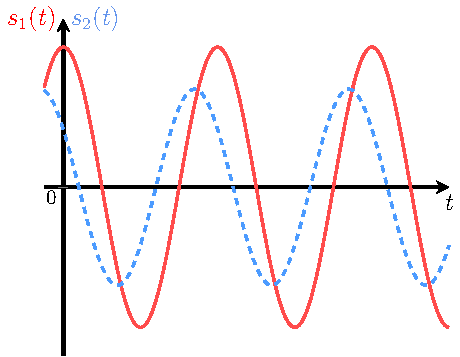
\includegraphics[width=\linewidth]{dfeqr}
% 		\captionsetup{justification=centering}
% 		\captionof{figure}{\\Déphasage}
% 	\end{center}
% \end{tcb*}

\subsection{Déphasage et différence de marche}
\subsubsection{Présentation}
Comme les fréquences sont les mêmes, le déphasage se réexprime par une
différence de distances.
\begin{tcb*}(prop){Déphasage et différence de marche}
	\vspace{-15pt}
	\begin{gather*}
		\beforetext{On a alors}
		\psw{\boxed{\D\f_{2/1}(\Mr) = -k\D L_{2/1}(\Mr) + \D\f_0}}
		\tag*{avec $\DS k = \frac{2\pi}{\lambda}$}
	\end{gather*}
	~
	\vspace{-15pt}
	\smallbreak
	\begin{isd}[interior hidden](prop)
		\tcbsubtitle{\fatbox{\textbf{Différence de marche}}}
		\psw{%
			\[
				\boxed{\Delta{L_{2/1}}(\Mr) = \SbMr - \SaMr}
			\]
		}%
		\vspace{-15pt}
		\tcblower
		\tcbsubtitle{\fatbox{\textbf{Déphasage à l'origine}}}
		\psw{%
			\[
				\boxed{\D\f_0 = \f_{02}-\f_{01}}
			\]
		}%
		\vspace{-15pt}
	\end{isd}
\end{tcb*}

\begin{tcb}(inte){Différence de marche}
	$\D L$ traduit la distance supplémentaire que doit parcourir une onde par
	rapport à une autre pour arriver au même point M. Comme elles vont à la même
	vitesse $c$ (même nature, même fréquence), cette distance supplémentaire
	introduit un retard de l'une par rapport à l'autre, c'est-à-dire un déphasage.
\end{tcb}

\begin{tcb}(demo)<lftt>{Différence de marche}
	\psw{%
		\[
			\Delta{\f}_{2/1}(\Mr) =
			-k\SbMr + \f_{02} - \pa{-k\SaMr + \f_{01}} =
			-k \pa{\SbMr - \SaMr} + \f_{02} - \f_{01}
		\]
	}%
	\vspace{-15pt}
\end{tcb}

\subsubsection{Valeurs particulières}
\begin{tcb*}(prop){$\Delta{L}$ particuliers}
	\textbf{Pour des sources de même phase à l'origine}, on a $\Delta{\f_0} = 0$.
	Les déphasages particuliers se réécrivent alors en termes de différence de
	marche, avec $p \in \Zb$~:
	\smallbreak
	\arrayrulecolor{prop}
	\begin{tabularx}{\linewidth}{l:Y:Y:Y}
		\textbf{Type}
		 &
		\textcolor{prop}{\fatbox{\textbf{En phase}}}
		 &
		\textcolor{prop}{\fatbox{\textbf{En quadrature}}}
		 &
		\textcolor{prop}{\fatbox{\textbf{En opposition}}}
		\\
		% \vspace{10pt}
		$\Delta{L}(\Mr)$
		 &
		\vspace{-15pt}
		\psw{%
			\[
				\boxed{p\lambda}
			\]
		}%
		\vspace{-15pt}
		 &
		\vspace{-15pt}
		\psw{%
			\[
				\boxed{\pa{p+\frac{1}{2}}\frac{\lambda}{2}}
			\]
		}%
		\vspace{-15pt}
		 &
		\vspace{-15pt}
		\psw{%
			\[
				\boxed{\pa{2p+1}\frac{\lambda}{2}}
			\]
		}%
		\vspace{-15pt}
	\end{tabularx}
\end{tcb*}

\begin{tcb*}(demo){$\Delta{L}$ particuliers}
	On part du lien entre $\Delta{\f}$ et $\Delta{L}$, avec $\Delta{\f_0} =
		0$, et de la définition du vecteur d'onde~:
	\psw{%
		\begin{gather*}
			\Delta{\f}(\Mr) = -k\Delta{L}(\Mr)
			\Lra
			\Delta{L}(\Mr) = -\Delta{\f}(\Mr) \frac{\lambda}{2\pi}
		\end{gather*}
	}%
	Comme $p \in \Zb$, $-p \in \Zb$, donc le signe $-$ importe peu. Ainsi,
	\begin{itemize}
		\item[b]{En phase}:
		      \vspace{-15pt}
		      \psw{%
			      \begin{gather*}
				      \Delta{L}(\Mr) = 2p\pi \cdot \frac{\lambda}{2\pi} = p\lambda
			      \end{gather*}
		      }%
		      \vspace{-25pt}
		\item[b]{En quadrature}:
		      \vspace{-15pt}
		      \psw{%
			      \begin{gather*}
				      \Delta{L}(\Mr) =
				      \pa{p+\frac{1}{2}}\pi \cdot \frac{\lambda}{2\pi} =
				      \pa{p+\frac{1}{2}}\frac{\lambda}{2}
			      \end{gather*}
		      }%
		      \vspace{-25pt}
		\item[b]{En opposition}:
		      \vspace{-15pt}
		      \psw{%
			      \begin{gather*}
				      \Delta{L}(\Mr) =
				      \pa{2p+1}\pi \cdot \frac{\lambda}{2\pi} =
				      \pa{2p+1}\frac{\lambda}{2}
			      \end{gather*}
		      }%
		      \vspace{-25pt}
	\end{itemize}
	\textbf{Tout fonctionne comme si on remplaçait $2\pi$ par $\lambda$}.
\end{tcb*}

\section{Superposition d'ondes sinusoïdales de mêmes fréquences}
\subsection{Présentation}

La plupart du temps, les ondes se croisent sans interagir particulièrement, et
on ne voit que la somme des signaux. Voir l'animation
\texttt{geogebra}\footnote{\url{https://www.geogebra.org/m/jyh2ZMXJ}}.
\begin{tcb}[sidebyside](exem)<lftt>{Superpositions sur une corde}
	\begin{center}
		\sswitch{%
			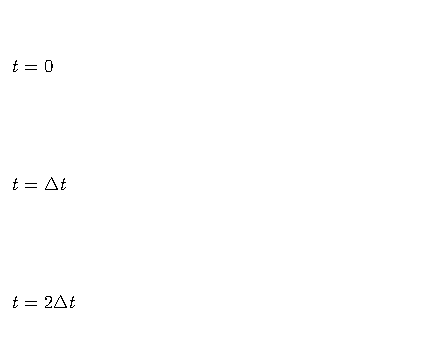
\includegraphics[width=.9\linewidth]{sum_pulse-cst_stud.pdf}
		}{%
			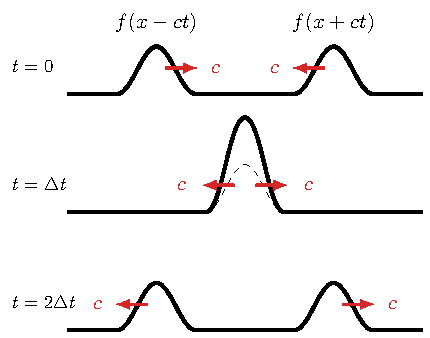
\includegraphics[width=.9\linewidth]{sum_pulse-cst_prof.pdf}
		}%
		\captionof{figure}{Mêmes amplitudes.}
	\end{center}
	\tcblower
	\begin{center}
		\sswitch{%
			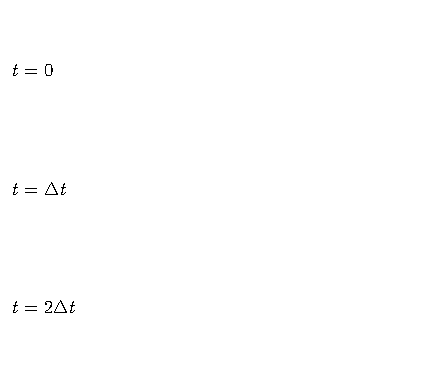
\includegraphics[width=.9\linewidth]{sum_pulse-dst_stud.pdf}
		}{%
			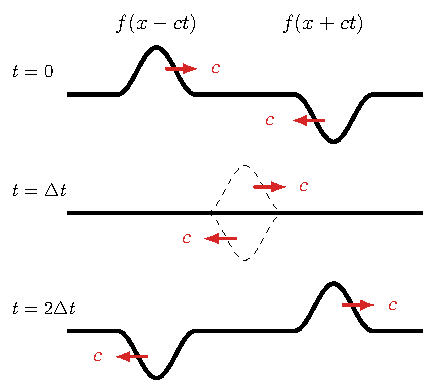
\includegraphics[width=.9\linewidth]{sum_pulse-dst_prof.pdf}
		}%
		\captionof{figure}{Amplitudes opposées.}
	\end{center}
\end{tcb}

Étudions mathématiquement ce phénomène en utilisant \textbf{deux sources
	sinusoïdales}.

\begin{tcb}[sidebyside, righthand ratio=.25](defi)<lftt>{Hypothèses}
	Chaque source émet une OPPS\ftn{Onde Plane Progressive Sinusoïdale}
	\textbf{de même fréquence} et \textbf{même nature} depuis les points
	$\Sr_1$ et $\Sr_2$~:
	\[
		\psw{s_1(\Mr,t) = A_1\cos(\wt+\f_1(\Mr))}
		\qet
		\psw{s_2(\Mr,t) = A_2\cos(\wt+\f_2(\Mr))}
	\]
	et on s'intéresse à leur somme $s(\Mr, t) = s_1(\Mr, t) + s_2(\Mr, t)$ en
	un point $\Mr$ de l'espace.
	\tcblower
	\begin{center}
		\sswitch{
			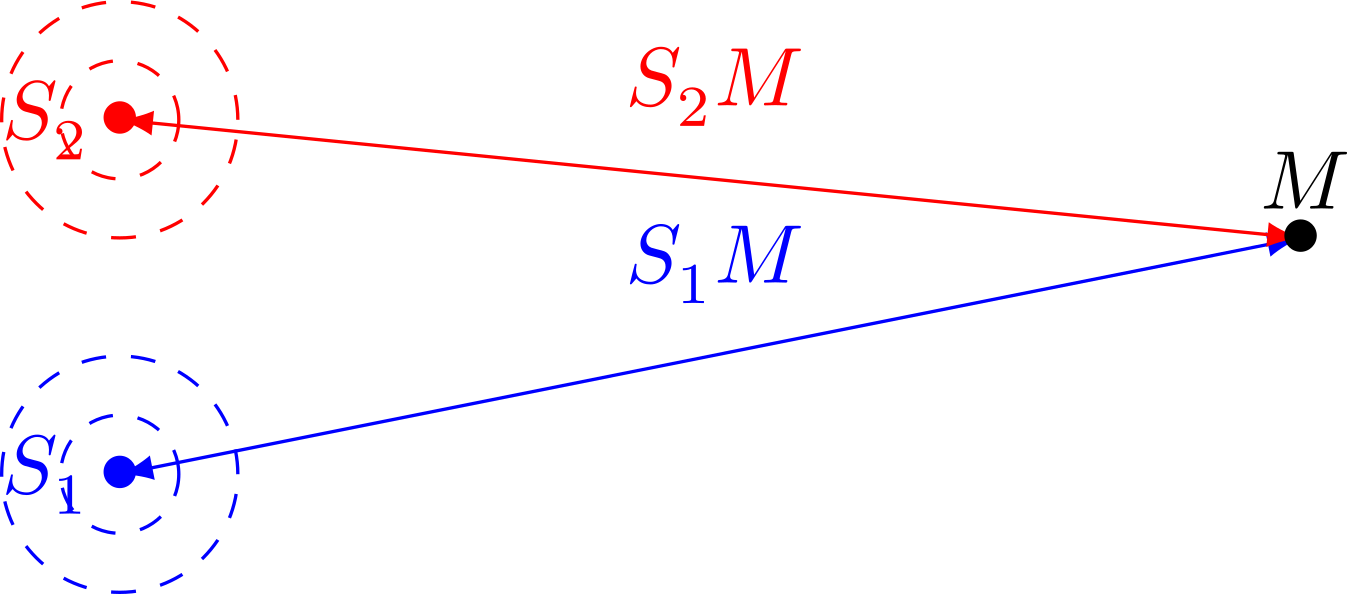
\includegraphics[width=\linewidth, draft=true]{S12M}
		}{
			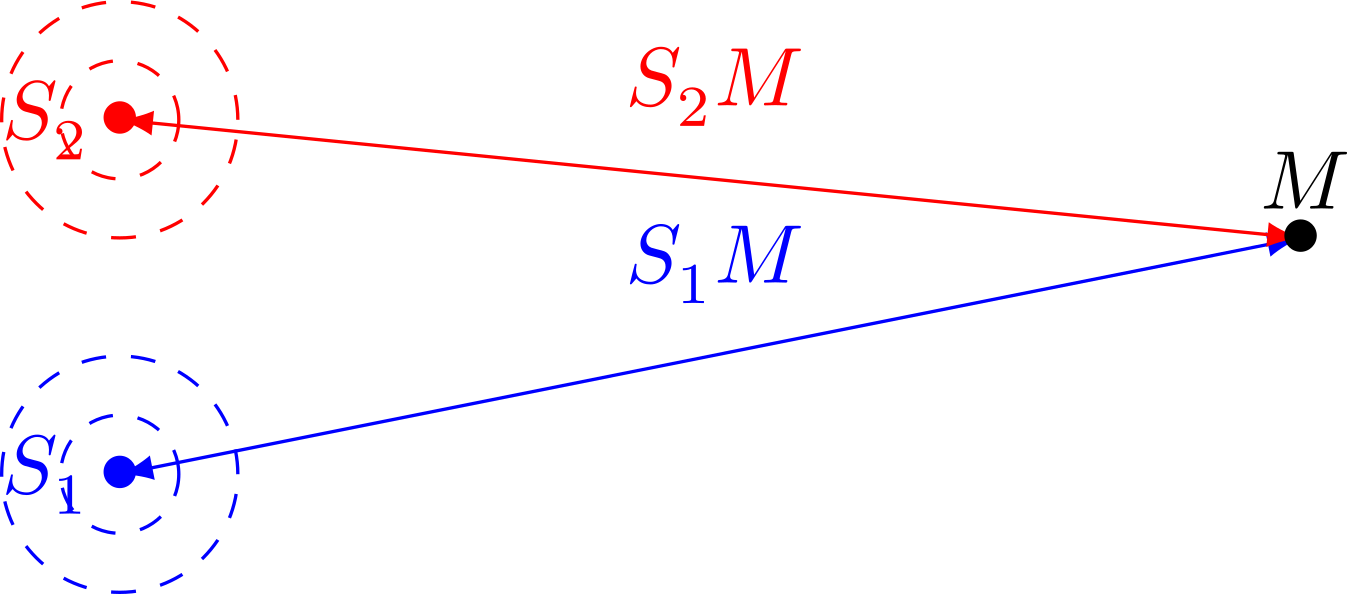
\includegraphics[width=\linewidth]{S12M}
		}
		\vspace{-15pt}
		\captionsetup{justification=centering}
		\captionof{figure}{\\Schéma.}
	\end{center}
\end{tcb}

\subsection{Signaux de même amplitude~: $A_1 = A_2 = A_0$}
\subsubsection{Cas général}

\begin{tcb}(tool)<lftt>{Somme de cosinus}
	On remplace la somme par un produit grâce à la relation
	\[
		\cos p + \cos q =
		2\cos( \frac{p-q}{2} )\cos ( \frac{p+q}{2} )
	\]
\end{tcb}

\begin{tcb*}[breakable](demo){Signal somme même amplitude}
	\vspace{-15pt}
	\psw{%
		\begin{align*}
			s(\Mr,t) & = s_1(\Mr,t) + s_2(\Mr,t)
			\\\Lra
			s(\Mr,t) & = A_0 \left[ \cos(\wt+\f_1(\Mr)) + \cos(\wt+\f_2(\Mr)) \right]
			\\\Lra
			s(\Mr,t) & = 2A_0
			\cos ( \frac{\wt + \f_1(\Mr) - \wt - \f_2(\Mr)}{2} )
			\cos ( \frac{\wt + \f_1(\Mr) + \wt + \f_2(\Mr)}{2} )
			\\\Lra
			s(\Mr,t) & = 2A_0
			\cos(\frac{\Delta{\f}_{2/1}(\Mr)}{2})
			\cos(\wt + \frac{\f_1(\Mr)+\f_2(\Mr)}{2})
		\end{align*}
	}%
\end{tcb*}

\begin{tcb}(prop){Signal somme même amplitude}
	\vspace{-15pt}
	\begin{gather*}
		\beforetext{Ainsi,}
		\psw{s(\Mr,t) = A(\Mr)\cos(\wt + \f(\Mr))}
		\tag*{avec}
	\end{gather*}
	~
	\vspace{-15pt}
	\smallbreak
	\begin{isd}[interior hidden](prop)
		\psw{%
			\[
				\boxed{A(\Mr) = 2A_0 \cos(\frac{\Delta{\f_{2/1}(\Mr)}}{2})}
			\]
		}%
		\vspace{-15pt}
		\tcblower
		\psw{%
			\[
				\boxed{\f(\Mr) = \frac{\f_1(\Mr)+\f_2(\Mr)}{2}}
			\]
		}%
		\vspace{-15pt}
	\end{isd}
\end{tcb}

\vspace{-10pt}
\subsubsection{Cas extrêmes}
\begin{tcb*}(prop){Cas extrêmes même amplitude}
	L'amplitude de $s(\Mr,t)$ est \textbf{maximale} pour des signaux \textbf{en phase}
	et \textbf{minimale} pour des signaux en \textbf{opposition de phase}, avec~:
	\smallbreak
	\begin{isd}[interior hidden](prop)
		\vspace{-15pt}
		\begin{gather*}
			\beforetext{\textcolor{prop}{\fatbox{\textbf{En phase}}}}
			\psw{\boxed{A\ind{max} = 2A_0}}
		\end{gather*}
		\vspace{-15pt}
		\tcblower
		\vspace{-15pt}
		\begin{gather*}
			\beforetext{\textcolor{prop}{\fatbox{\textbf{En opposition}}}}
			\qquad
			\psw{\boxed{A\ind{min} = 0}}
		\end{gather*}
		\vspace{-15pt}
	\end{isd}
\end{tcb*}

\begin{tcb*}[breakable](demo){Cas extrêmes même amplitude}
	\tcbsubtitle{\fatbox{\textbf{Amplitude maximale}}}
	\vspace{-15pt}
	\begin{gather*}
		\beforetext{$A(\Mr)$ est maximale pour}
		\psw{%
			\cos ( \frac{\D\f_{2/1}(\Mr)}{2} ) = \pm 1
			\Ra
			A\ind{max} = 2A_0
		}%
		\\\beforetext{$\Ra$}
		\psw{%
			\cos \left( \frac{\D\f_{2/1}(\Mr)}{2} \right) = \pm 1
			\quad \Lra \quad
			\frac{\D\f_{2/1}(\Mr)}{2} = p\pi
			\quad \Lra \quad
			\D\f_{2/1}(\Mr) = 2p\pi
			\tag*{$p \in \Zb$}
		}%
	\end{gather*}
	Ce déphasage correspond à des \textbf{signaux en phase}. Lorsque
	les signaux sont en phase, les maxima et minima de vibration se correspondent
	et donnent à chaque instant une amplitude double.
	\tcblower
	\tcbsubtitle{\fatbox{\textbf{Amplitude minimale}}}
	\vspace{-15pt}
	\begin{gather*}
		\beforetext{$A(\Mr)$ est minimale pour}
		\psw{%
			\cos ( \frac{\D\f_{2/1}(\Mr)}{2} ) = 0
			\Ra
			A\ind{min} = 0
		}%
		\\\beforetext{$\Ra$}
		\psw{%
			\cos \left( \frac{\D\f_{2/1}(\Mr)}{2} \right) = 0
			\quad \Lra \quad
			\frac{\D\f_{2/1}(\Mr)}{2} = p\pi + \frac{\pi}{2}
			\quad \Lra \quad
			\D\f_{2/1}(\Mr) = (2p+1)\pi
			\tag*{$p \in \Zb$}
		}%
	\end{gather*}
	Ce sont donc des \textbf{signaux en opposition de phase}. Lorsque
	les signaux sont en opposition de phase, les maxima et minima de vibration
	s'opposent, et l'amplitude résultante est nulle.
\end{tcb*}

\subsubsection{Conclusion}
\begin{tcb}[breakable](ror){Analyse même amplitude}
	Le signal somme de deux OPPS de \textbf{même amplitude} $A_0$ et \textbf{même
		pulsation} $\w$ est~:
	\begin{enumerate}
		\item Un signal \textbf{sinusoïdal} et \textbf{de même pulsation
			      $\mathbf{\w}$}~;
		\item D'amplitude \textbf{dépendante de M}, et
		      \begin{itemize}
			      \item \textbf{Maximale} $A\ind{max} = 2A_0$ pour signaux \textbf{en
				            phase} ($\D\f_{2/1} = 2p\pi$, $p\in\Zb$)~;
			      \item \textbf{Minimale} $A\ind{min} = 0$ pour signaux \textbf{en
			            opposition de phase} ($\D\f_{2/1} = (2p+1)\pi$, $p\in\Zb$).
		      \end{itemize}
	\end{enumerate}
	\begin{isd}
		\begin{center}
			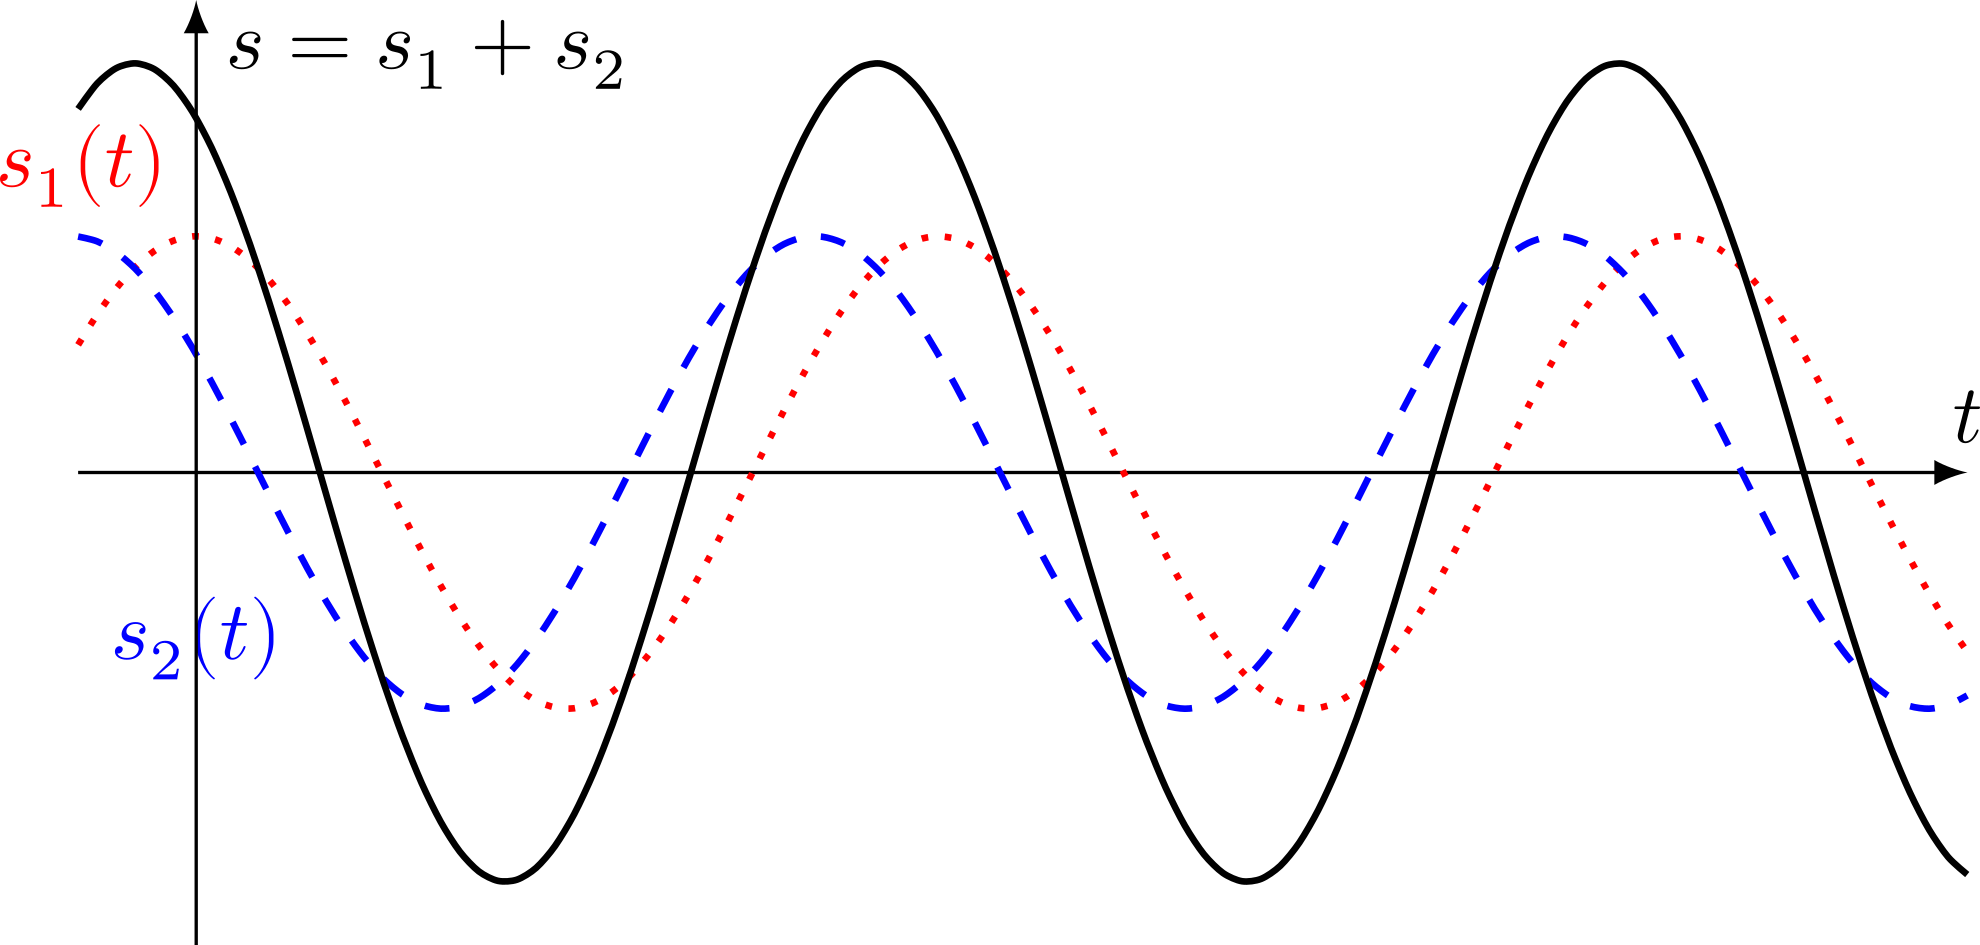
\includegraphics[width=\linewidth]{somme_pi3}
			\captionsetup{justification=centering}
			\captionof{figure}{\\Somme avec déphasage $\D\f_{2/1} = \pi/3$.}
			\label{fig:sommepi3}
		\end{center}
		\tcblower
		\begin{center}
			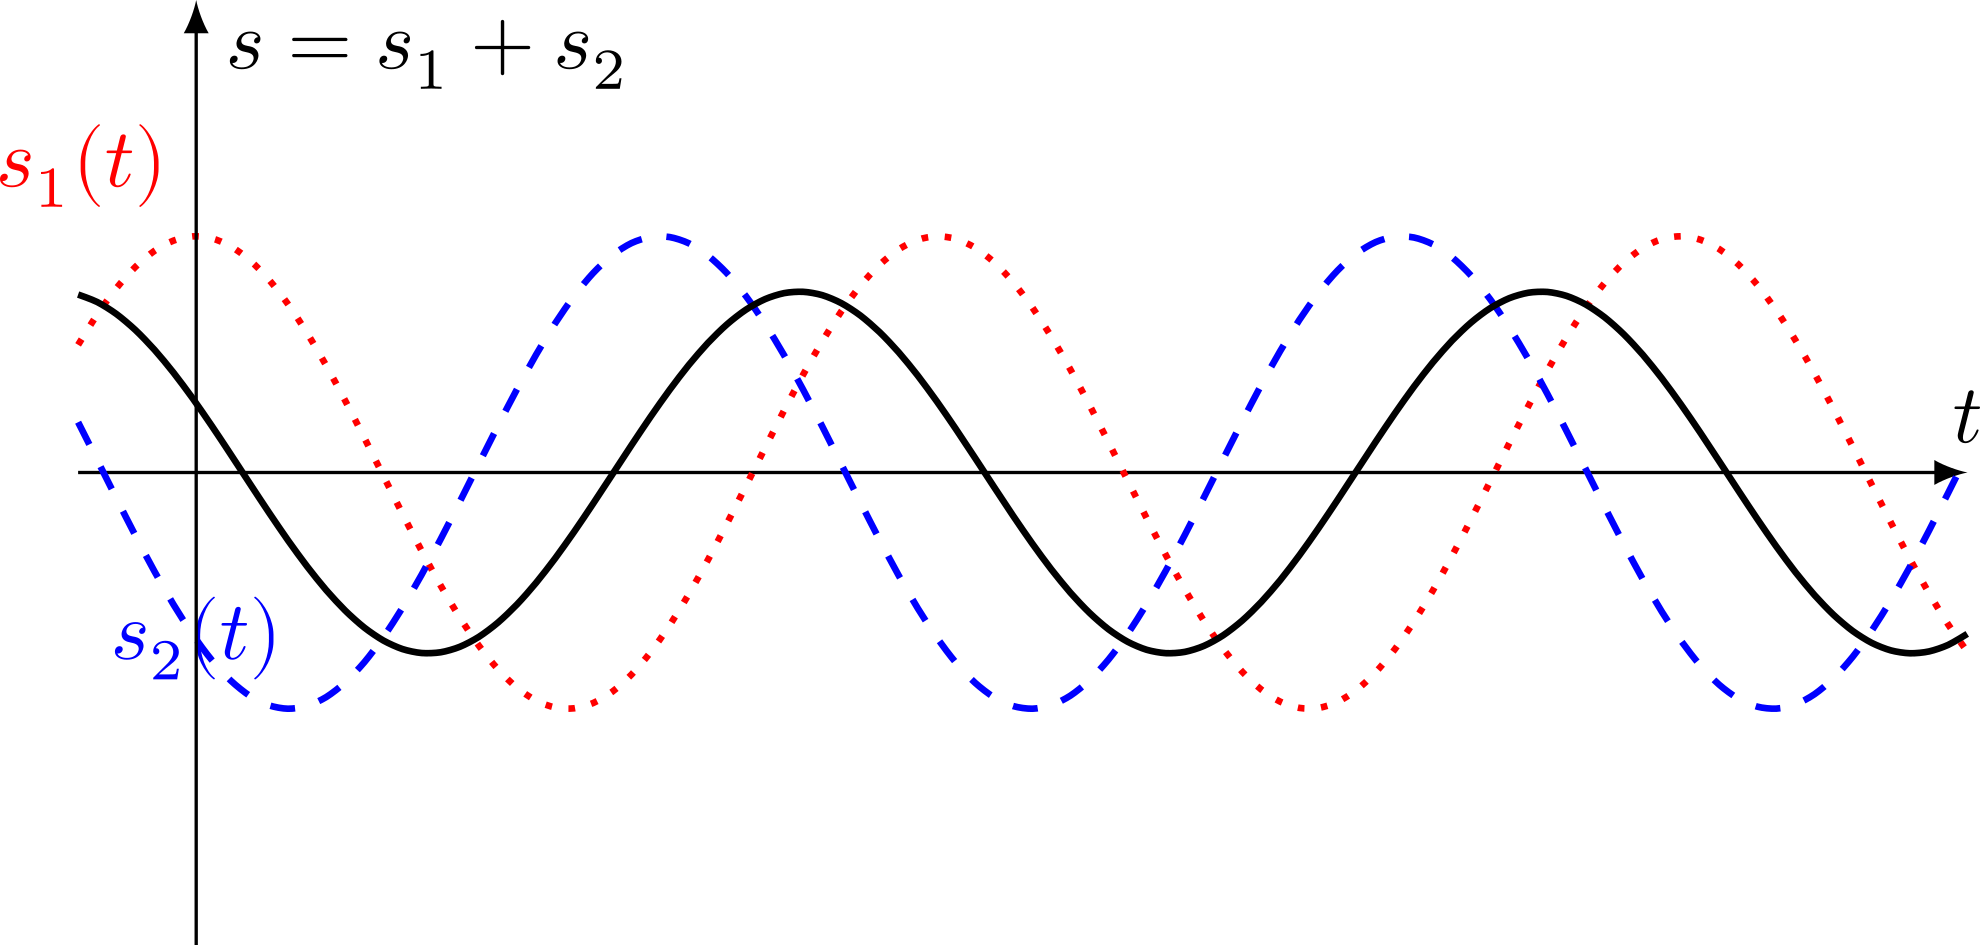
\includegraphics[width=\linewidth]{somme_3pi4}
			\captionsetup{justification=centering}
			\captionof{figure}{\\Somme avec déphasage $\D\f_{2/1} = 3\pi/4$.}
			\label{fig:somme3pi4}
		\end{center}
	\end{isd}
\end{tcb}

\subsection{Signaux d'amplitudes différentes~: $A_1 \neq A_2$}
\subsubsection{Cas général}
On peut soit utiliser la trigonométrie classique, soit les complexes~:
\begin{tcb}[sidebyside](tool)<lftt>{Trigonométrie}
	\vspace*{-15pt}
	\begin{align*}
		\cos(a+b) & = \cos a\cos b - \sin a\sin b \\
		\cos(a-b) & = \cos a\cos b + \sin a\sin b
	\end{align*}
	\tcblower
	\vspace*{-15pt}
	\begin{gather*}
		\cos\theta = \frac{\exr^{\jj\theta}+\exr^{-\jj\theta}}{2}\\
		\abs{\zu}^2 = \zu\cdot\zu^*
		\qet
		\tan (\arg*{\zu}) = \frac{\Im(\zu)}{\Re(\zu)}
	\end{gather*}
\end{tcb}

\begin{tcb}(prop){Signal somme amplitudes $\neq$}
	\vspace{-15pt}
	\begin{gather*}
		\beforetext{Ainsi,}
		\psw{s(\Mr,t) = A(\Mr)\cos(\wt + \f(\Mr))}
		\tag*{avec}
	\end{gather*}
	~
	\vspace{-15pt}
	\smallbreak
	\begin{isd}[interior hidden](prop)
		\vspace{-15pt}
		\psw{%
		\[
			\small
			\boxed{%
			A(\Mr) = \sqrt{A_1{}^2+A_2{}^2 + 2A_1A_2\cos(\D\f_{2/1}(\Mr))
			}
			}
		\]
		}%
		\vspace{-15pt}
		\tcblower
		\vspace{-15pt}
		\psw{%
			\[
				\small
				\boxed{%
					\f(\Mr) = \arctan(
					\dfrac{%
						A_1\sin\f_1(\Mr)+A_2\sin\f_2(\Mr)
					}{
						A_1\cos\f_1(\Mr)+A_2\cos\f_2(\Mr)
					}
					)
				}
			\]
		}%
		\vspace{-15pt}
	\end{isd}
\end{tcb}

\begin{tcb}[breakable](demo){Signal somme amplitudes $\neq$}
	\tcbsubtitle{\fatbox{En réels}}
	\vspace{-20pt}
	\psw{%
		\begin{align*}
			s(\Mr,t)                & = A_1\cos(\wt+\f_1(\Mr)) + A_2\cos(\wt+\f_2(\Mr))
			\\\Lra
			s(\Mr,t)                & =
			A_1(\cos (\wt)\cos (\f_1(\Mr)) - \sin (\wt)\sin (\f_1(\Mr)))
			\\
			                        & +
			A_2(\cos (\wt)\cos (\f_2(\Mr)) - \sin (\wt)\sin (\f_2(\Mr)))
			\\\Lra
			s(\Mr,t)                & =
			(A_1\cos (\f_1(\Mr))+A_2\cos (\f_2(\Mr)))\cos (\wt)
			\\
			                        & -
			(A_1\sin (\f_1(\Mr))+A_2\sin (\f_2(\Mr)))\sin (\wt)
			\\\Lra
			\Aboxed{s(\Mr,t)        & = A(\Mr)\cos(\wt+\f(\Mr))}
			\\\beforetext{car}
			A(\Mr)\cos(\wt+\f(\Mr)) & =
			A(\Mr)\cos (\f(\Mr))\cos (\wt) -
			A(\Mr)\sin (\f(\Mr))\sin (\wt)
		\end{align*}
		On trouve donc
		\[
			\left\{
			\begin{array}{rcl}
				A(\Mr)\cos\f(\Mr) & = & A_1\cos\f_1(\Mr) + A_2\cos\f_2(\Mr)
				\hspace{\fill}
				(1)
				\\
				A(\Mr)\sin\f(\Mr) & = & A_1\sin\f_1(\Mr) + A_2\sin\f_2(\Mr)
				\hspace{\fill}
				(2)
			\end{array}
			\right.
		\]
		On obtient $A(\Mr)$ l'amplitude de l'onde somme en prenant $(1)^2+(2)^2$, et
		$\tan\f(\Mr)$ avec $(2)/(1)$~:
	}%

	\psw{%
		\begin{gather*}
			\small
			\left\{
			\begin{array}{rcl}
				A(\Mr)^2\underbracket[1pt]{(\cos^2\f(\Mr) + \sin^2\f(\Mr))}_{=1}
				            & = &
				A_1{}^2 + A_2{}^2 + 2A_1A_2
				\underbracket[1pt]{%
					(\cos\f_1(\Mr)\cos\f_2(\Mr) + \sin\f_1(\Mr)\sin\f_2(\Mr))
				}_{=\cos(\f_1(\Mr)-\f_2(\Mr))}
				\\[2em]
				\tan\f(\Mr) & = &
				\dfrac{%
					A_1\sin\f_1(\Mr)+A_2\sin\f_2(\Mr)
				}{
					A_1\cos\f_1(\Mr)+A_2\cos\f_2(\Mr)
				}
			\end{array}
			\right.
			% \\[1em]
			% \Leftrightarrow
			% \left\{
			% \begin{array}{rcl}
			%   A(\Mr) & = & \sqrt{A_1{}^2+A_2{}^2 + 2A_1A_2\cos(\D\f_{2/1})} \\
			%   \f(\Mr) & = & \arctan (
			%     \dfrac{%
			%       A_1\sin\f_1(\Mr)+A_2\sin\f_2(\Mr)
			%     }{%
			%       A_1\cos\f_1(\Mr)+A_2\cos\f_2(\Mr)
			%     }
			%   )
			% \end{array}
			% \right.
		\end{gather*}
	}
	\vspace{-10pt}
	\tcblower
	\tcbsubtitle{\fatbox{En complexes}}
	En supposant directement que $s(\Mr,t) = A(\Mr)\cos(\wt+\f(\Mr))$ (par
	linéarité),
	\psw{%
		\begin{gather*}
			\begin{aligned}
				\xul{s}(\Mr,t)                                & =
				\xul{s_1}(\Mr,t) + \xul{s_2}(\Mr,t)
				\\ \Lra
				A(\Mr)\exr^{\jj\f(\Mr)}\cancel{\exr^{\jj\wt}} & =
				A_1\exr^{\jj\f_1(\Mr)}\cancel{\exr^{\jj\wt}} +
				A_2\exr^{\jj\f_2(\Mr)}\cancel{\exr^{\jj\wt}}
				\\ \Lra
				A(\Mr)\exr^{\jj\f(\Mr)}                       & =
				A_1\exr^{\jj\f_1(\Mr)} +
				A_2\exr^{\jj\f_2(\Mr)}
			\end{aligned}\\
			\begin{aligned}
				\Ra
				 &
				\left\{
				\begin{array}{rcl}
					\abs{\xul{A}(\Mr)}^2 & = &
					\xul{A}(\Mr) \cdot \xul{A}^*(\Mr) =
					(\xul{A_1}+\xul{A_2})(\xul{A_1}^* + \xul{A_2}^*)
					\\
					\arg*{\xul{A}}       & = & \arg*{\xul{A_1}+\xul{A_2}}
				\end{array}
				\right.
				\\ \Lra
				 &
				\left\{
				\begin{array}{rcl}
					A(\Mr)^2 & = &
					(A_1\exr^{\jj\f_1(\Mr)}+A_2\exr^{\jj\f_2(\Mr)}) \cdot
					(A_1\exr^{-\jj\f_1(\Mr)}+A_2\exr^{-\jj\f_2(\Mr)})
					\\
					\f(\Mr)  & = &
					\arg*{%
						A_1\cos\f_1(\Mr)+ \jj A_1\sin\f_1(\Mr) +
						A_2\cos\f_2(\Mr) + \jj A_2\sin\f_2(\Mr))
					}
					\\
				\end{array}
				\right.
				\\ \Lra &
				\small
				\left\{
				\begin{array}{rcl}
					A(\Mr)^2    & = & A_1{}^2
					\underbracket[1pt]{\exr^{\jj(\f_1(\Mr)-\f_1(\Mr))}}_{=1} +
					A_2{}^2
					\underbracket[1pt]{\exr^{\jj(\f_2(\Mr)-\f_2(\Mr))}}_{=1} +
					A_1A_2
					\underbracket{%
						\left(
						\exr^{\jj(\f_1(\Mr)-\f_2(\Mr))} + \exr^{-\jj(\f_1(\Mr)-\f_2(\Mr))}
						\right)
					}_{=2\cos\D\f_{2/1}(\Mr)}
					\\[2em]
					\tan\f(\Mr) & = &
					\dfrac{%
						A_1\sin\f_1(\Mr)+A_2\sin\f_2(\Mr)
					}{
						A_1\cos\f_1(\Mr)+A_2\cos\f_2(\Mr)
					}
				\end{array}
				\right.
				% \\ \Lra &
				% \left\{
				% \begin{array}{rcl}
				%   A(\Mr) & = & \sqrt{A_1{}^2+A_2{}^2 + 2A_1A_2\cos(\D\f_{2/1}(\Mr))} \\
				%   \f(\Mr) & = & \arctan(
				%   \dfrac{%
				%     A_1\sin\f_1(\Mr)+A_2\sin\f_2(\Mr)
				%   }{
				%     A_1\cos\f_1(\Mr)+A_2\cos\f_2(\Mr)
				%   }
				%   )
				% \end{array}
				% \right.
			\end{aligned}
		\end{gather*}}
	\hspace{-20pt}
	\hdashrule[0.5ex]{1.05\linewidth}{.5pt}{3pt}
	\vspace{-15pt}
	\begin{gather*}
		\beforetext{Dans tous les cas, on trouve}
		\hspace{80pt}
		\left\{
		\begin{array}{rcl}
			A(\Mr)  & = & \sqrt{A_1{}^2+A_2{}^2 + 2A_1A_2\cos(\D\f_{2/1}(\Mr))}
			\\
			\f(\Mr) & = & \arctan(
			\dfrac{%
					A_1\sin\f_1(\Mr)+A_2\sin\f_2(\Mr)
				}{
					A_1\cos\f_1(\Mr)+A_2\cos\f_2(\Mr)
				}
			)
		\end{array}
		\right.
	\end{gather*}
\end{tcb}

% Ainsi, même si les amplitudes sont différentes le résultat fondamental reste le
% même~: l'amplitude dépend du déphasage et il y a possibilité d'avoir des
% interférences constructives et destructives. Les minima et maxima ne sont
% cependant \textbf{plus les mêmes}.

\subsubsection{Cas extrêmes}
\begin{tcb*}(prop){Cas extrêmes amplitudes $\neq$}
	L'amplitude de $s(\Mr,t)$ est \textbf{maximale} pour des signaux \textbf{en
		phase} et \textbf{minimale} pour des signaux en \textbf{opposition de phase},
	avec~:
	\smallbreak
	\begin{isd}[interior hidden](prop)
		\vspace{-15pt}
		\begin{gather*}
			\beforetext{\textcolor{prop}{\fatbox{\textbf{En phase}}}}
			\psw{\boxed{A\ind{max} = A_1+A_2}}
		\end{gather*}
		\vspace{-15pt}
		\tcblower
		\vspace{-15pt}
		\begin{gather*}
			\beforetext{\textcolor{prop}{\fatbox{\textbf{En opposition}}}}
			\hspace{60pt}
			\psw{\boxed{A\ind{min} = \abs{A_1-A_2}}}
		\end{gather*}
		\vspace{-15pt}
	\end{isd}
\end{tcb*}

\begin{tcb*}[breakable](demo){Cas extrêmes amplitudes $\neq$}
	\tcbsubtitle{\fatbox{\textbf{Amplitude maximale}}}
	\vspace{-15pt}
	\begin{gather*}
		\beforetext{Max pour}
		\psw{%
		\cos (\D\f_{2/1}(\Mr)) = 1
		\Ra
		A\ind{max} = \sqrt{A_1{}^2 + A_2{}^2 + 2A_1A_2} = A_1+A_2
		}%
		\\\beforetext{$\Ra$}
		\psw{%
			\cos (\D\f_{2/1}(\Mr)) = 1
			\quad \Lra \quad
			\D\f_{2/1}(\Mr) = 2p\pi
			\tag*{$p \in \Zb$}
		}%
	\end{gather*}
	% Ce sont donc des \textbf{signaux en phase}.
	\tcblower
	\tcbsubtitle{\fatbox{\textbf{Amplitude minimale}}}
	\vspace{-15pt}
	\begin{gather*}
		\beforetext{Min pour}
		\psw{%
		\cos (\D\f_{2/1}(\Mr)) = 1
		\Ra
		A\ind{min} = \sqrt{A_1{}^2 + A_2{}^2 - 2A_1A_2} = A_1-A_2
		}%
		\\\beforetext{$\Ra$}
		\psw{%
			\cos (\D\f_{2/1}(\Mr)) = -1
			\quad \Lra \quad
			\D\f_{2/1}(\Mr) = (2p+1)\pi
			\tag*{$p \in \Zb$}
		}%
	\end{gather*}
	% Ce sont donc des \textbf{signaux en opposition de phase}.
\end{tcb*}

\subsubsection{Conclusion}
\begin{tcb}(ror){Analyse amplitudes différentes}
	Le signal somme de deux OPPS d'amplitudes $A_1$ et $A_2$ de même pulsation
	$\w$ est~:
	\begin{enumerate}
		\item Un signal \textbf{sinusoïdal} et \textbf{de même pulsation
			      $\mathbf{\w}$}~;
		\item D'amplitude \textbf{dépendante de M}, et
		      \begin{itemize}
			      \item \textbf{Maximale} $A\ind{max} = A_1 + A_2$ pour signaux
			            \textbf{en phase} ($\D\f_{2/1} = 2p\pi$)~;
			      \item \textbf{Minimale} $A\ind{min} = \abs{A_1 - A_2}$ pour signaux
			            \textbf{en opposition de phase} ($\D\f_{2/1} = (2p+1)\pi$).
		      \end{itemize}
	\end{enumerate}
	\begin{isd}
		\begin{center}
			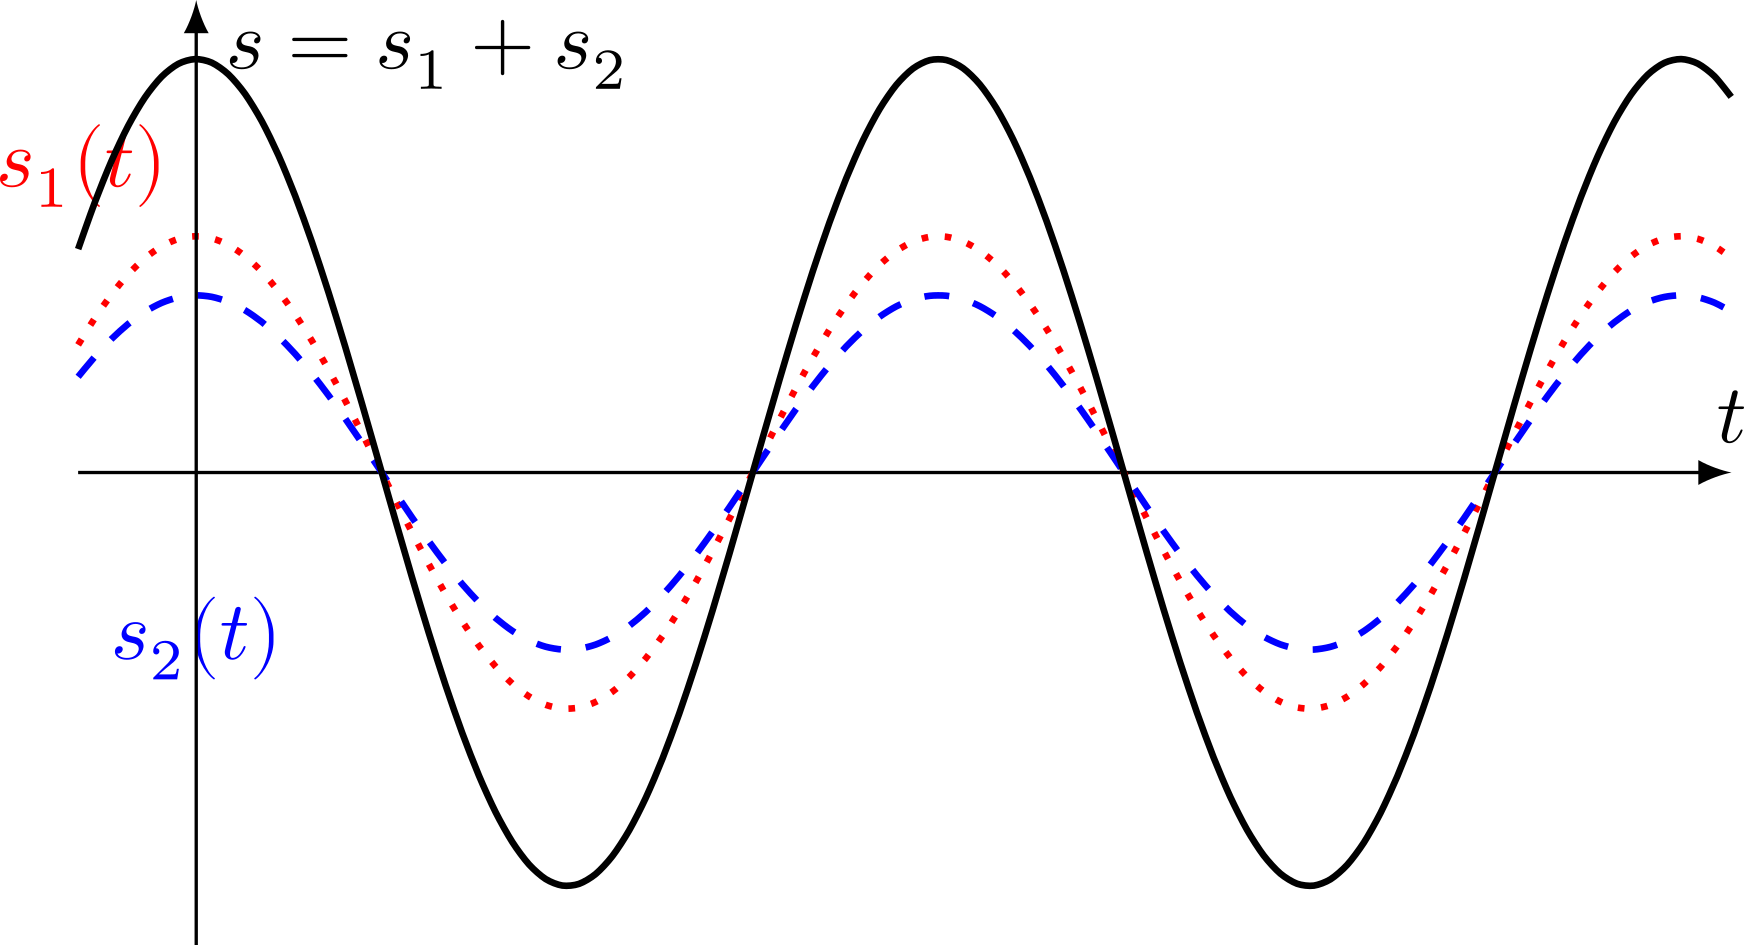
\includegraphics[width=\linewidth]{somme_0}
			\captionof{figure}{Signaux en phase.}
			\label{fig:sommephase}
		\end{center}
		\tcblower
		\begin{center}
			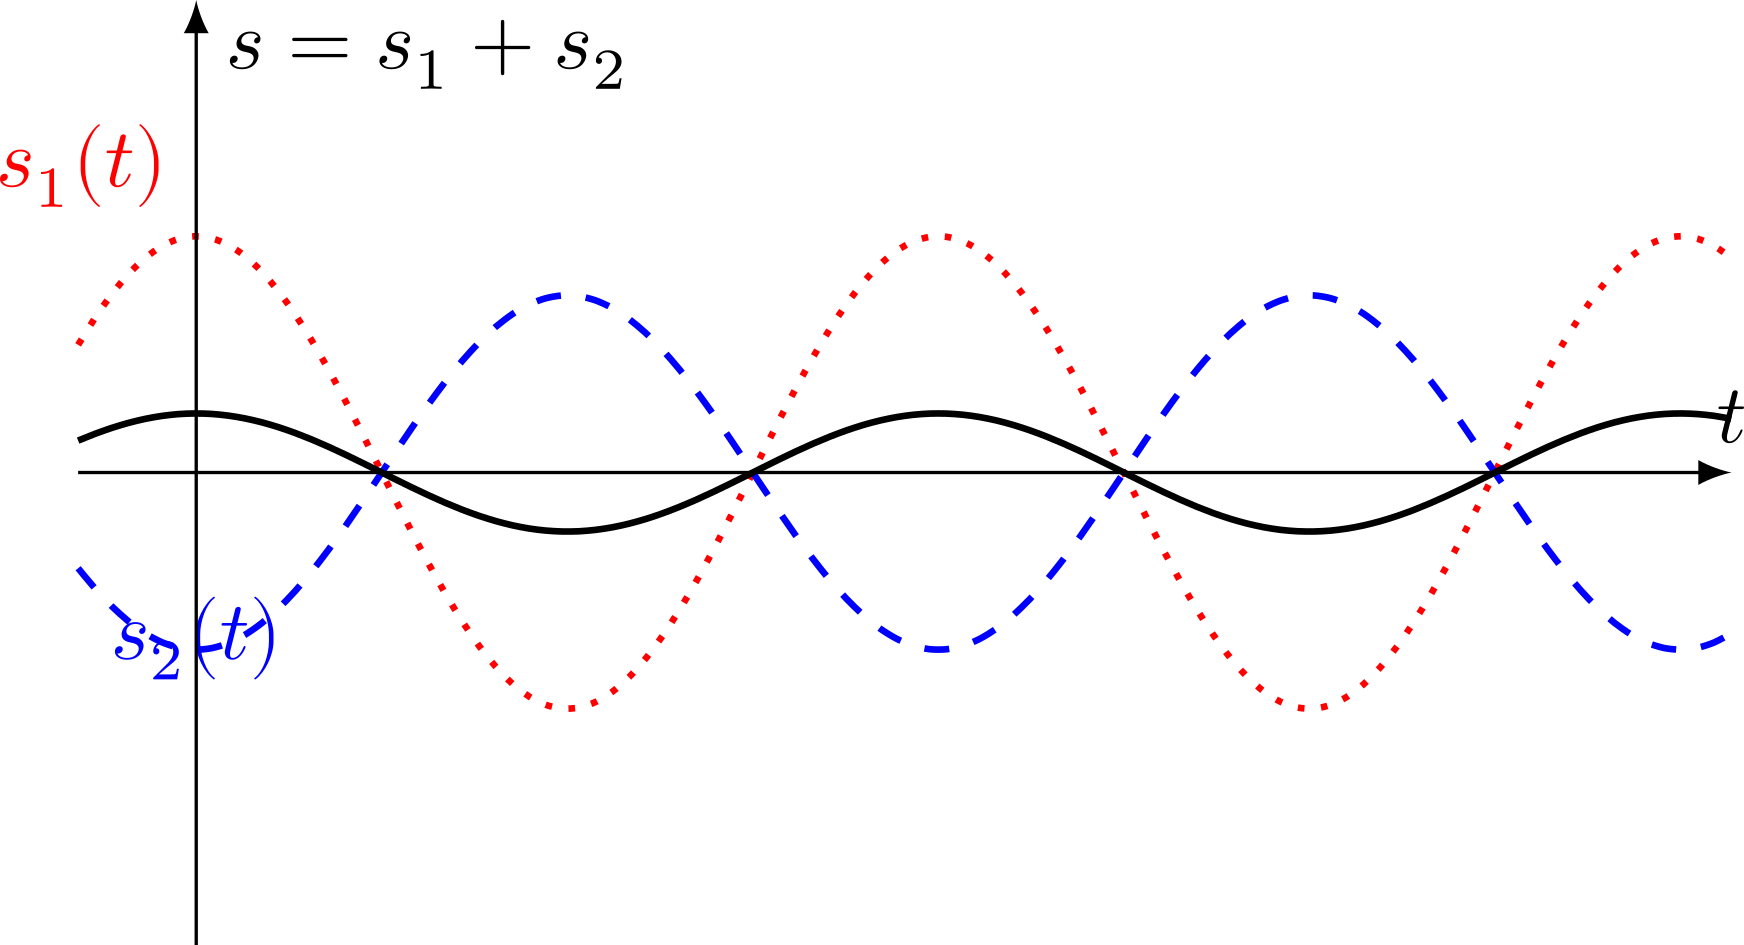
\includegraphics[width=\linewidth]{somme_pi}
			\captionof{figure}{Signaux en opposition.}
			\label{fig:sommeopp}
		\end{center}
	\end{isd}
\end{tcb}

\subsection{Bilan}

\begin{tcb}[breakable](ror){Interférences (pour $\Delta{\f_0} = 0$)}
	Pour deux OPPS \textbf{de même fréquence}, \textbf{nature} et \textbf{phase à
		l'origine}$^*$ se superposant en M~:
	\begin{isd}
		L'amplitude de la somme est \textbf{maximale} si les signaux sont
		\textbf{en phase}~:
		\[
			\boxed{\D\f_{2/1}(\Mr) = 2p\pi}
			\quad \stc{\Lra}{*} \quad
			\boxed{\Delta{L}_{2/1}(\Mr) = p\lambda}
		\]
		On parle d'\textbf{interférences constructives}.
		\tcblower
		L'amplitude de la somme est \textbf{minimale} si les signaux sont
		\textbf{en opposition de phase}~:
		\[
			\footnotesize
			\hspace*{-15pt}
			\boxed{\D\f_{2/1}(\Mr) = (2p+1)\pi}
			\quad  \stc{\Lra}{*} \quad
			\boxed{\Delta{L}_{2/1}(\Mr) = (2p+1)\frac{\lambda}{2}}
		\]
		On parle d'\textbf{interférences destructives}.
	\end{isd}
	\centering$p\in\Zb$ est appelé l'\textbf{ordre d'interférence}\ftn{Pour une
		animation et visualisation dans le plan, voir
		\href{https://phyanim.sciences.univ-nantes.fr/Ondes/cuve_ondes/interference_ondes_circulaires.php}{ce
			site}.}.
\end{tcb}

\begin{tcb*}[breakable](appl)<lftt>{Interférences sonores}
	\begin{minipage}{0.60\linewidth}
		Soient 2 émetteurs sonores envoyant une onde progressive sinusoïdale de même
		fréquence, même amplitude et \textbf{même phase à l'origine}.
		Le premier est fixé à l'origine du repère, l'émetteur 2 est mobile et à une
		distance $d$ du premier, et un microphone est placé à une distance fixe
		$x_0$ de l'émetteur 1 et est aligné avec les deux émetteurs.
	\end{minipage}
	\hfill
	\begin{minipage}{0.40\linewidth}
		\begin{center}
			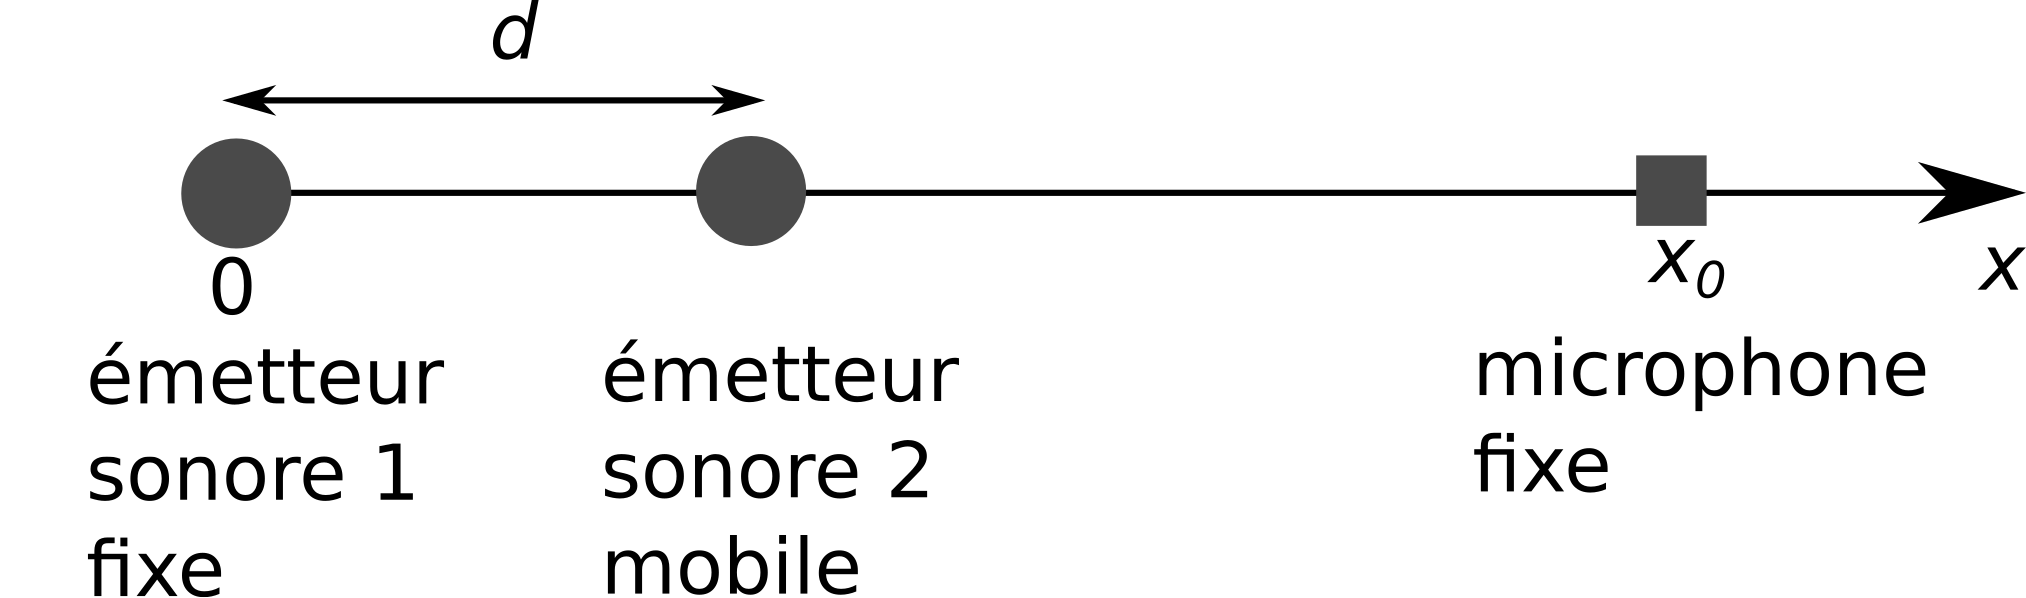
\includegraphics[width=\linewidth]{microphone}
		\end{center}
	\end{minipage}
	\smallbreak
	On néglige l'influence de l'émetteur 2 sur l'émetteur 1 et toute atténuation.
	\begin{enumerate}[label=\sqenumi]
		\item Lorsque $d=0$, qu'enregistre-t-on au niveau du microphone~?
		\item On part de $d=0$ et on augmente $d$ jusqu'à ce que le signal
		      enregistré soit nul. Ceci se produit pour $d = \SI{6.0}{cm}$.
		      Expliquer cette extinction.
		\item En déduire la longueur d'onde du son émis.
		\item Pour $d = \SI{12.0}{cm}$, quelle sera l'amplitude du signal
		      enregistré ?
	\end{enumerate}
	\tcblower
	\psw{
		\begin{enumerate}[label=\sqenumi]
			\item Si $d = 0$, alors la différence de marche $\D L_{1/2}(x_0) = 0$~; de
			      plus, comme les phases à l'origine des temps de chaque source est la
			      même, on a $\D\f_0 = 0$~: ainsi, on a
			      \[\boxed{\D\f_{1/2}(x_0) = 0}\]
			      Autrement dit, les signaux sont en phase. Comme ils ont la même
			      amplitude, au microphone on enregistre un signal de la fréquence
			      d'émission, avec une amplitude double de celle d'un émetteur.
			\item On a toujours $\D\f_0 = 0$, donc $\D\f_{1/2}(x_0) = -k\D
				      L_{1/2}(x_0)$. En augmentant la distance entre les sources, on
			      augmente le déphasage (en valeur absolue), en mettant la source 1 en
			      retard par rapport à la 2. Ainsi, il y a une valeur de différence de
			      marche telle que $\D\f_{1/2}(x_0) = -\pi$, c'est-à-dire que les
			      signaux seront en opposition de phase et s'annuleront.
			\item ~
			      \vspace{-24pt}
			      \begin{align*}
				      \D L_{1/2}(x_0) & = \SaMr - \SbMr = d
				      \\ \Lra
				      \D\f_{1/2}(x_0) & = -k\D L_{1/2} = -kd
				      \\ \Lra
				      -\pi            & = - \frac{2\pi}{\lambda}d \\
				      \Leftrightarrow
				      \Aboxed{\lambda & = 2d}
				      \qavec
				      d = \SI{6.0}{cm}
				      \\
				      \AN
				      \makebox[0pt][l]{$\xul{\phantom{\lambda = \SI{12.0}{cm}}}$}
				      \lambda         & = \SI{12.0}{cm}
			      \end{align*}
			      Les émetteurs émettent dans les micro-ondes.
			\item Si on double la distance, alors on aura $\D\f_{1/2}(x_0) = -2kd =
				      -2\pi$~: ceci est congru à 0 modulo $2\pi$, donc les signaux
			      seront de nouveau en phase, et on récupère le signal trouvé
			      question
			      \fbox{1}.
		\end{enumerate}
	}
	\vspace{-15pt}
\end{tcb*}

\section{Interférences lumineuses}
\subsection{Cohérence d'ondes lumineuses}

\begin{tcb}[breakable](defi){Cohérence entre sources}
	La plupart des sources lumineuses ont une phase à l'origine qui \textbf{n'est
		pas constante}, mais prend une valeur aléatoire au bout d'un certain temps
	généralement très court~: on dit qu'elles envoient des \textbf{trains
		d'ondes}. On définit ainsi~:
	\begin{itemize}
		\item[b]{Temps de cohérence}~: \psw{$\tau_c$, durée pour laquelle $\f_0 =
				      \cte$. Après $\tau_c$, le prochain train d'onde a un autre
			      $\f_0$.}
		\item[b]{Longueur de cohérence}~: \psw{$L_c = c\tau_c$, c'est la distance de
			      cohérence d'un train d'onde, i.e.\ avec une unique phase à
			      l'origine.} \end{itemize}
	% \smallbreak
	% On appelle cette durée le \textbf{temps de cohérence} et on la note
	% $\tau_c$~;
	% elle correspond à la durée sur laquelle l'onde émise par une source a une
	% phase à l'origine des temps constante, c'est-à-dire $\f_0 = \cte$. Après
	% $\tau_c$, le prochain train d'onde émis par la source a une autre valeur de
	% phase à l'origine des temps.
	% \smallbreak
	% On peut également parler de \textbf{longueur de cohérence} $L_c = c\tau_c$~:
	% c'est la distance sur laquelle un train d'onde est cohérent, c'est-à-dire
	% avec
	% une unique phase à l'origine.
\end{tcb}

\begin{tcb*}(prop){Condition d'interférence}
	Pour interférer, \textbf{deux sources doivent être cohérentes}, c'est-à-dire
	avoir $\D\f_0 = \cte$~; ceci n'est en général pas réalisable par manque de
	contrôle sur cette variation de phase à l'origine, et les interférences
	lumineuses se font donc \textbf{avec une unique source}, donnant forcément des
	ondes cohérentes.
\end{tcb*}

\begin{tcb}[sidebyside, lefthand ratio=.4](exem)<lftt>{Cohérence}
	\begin{center}
		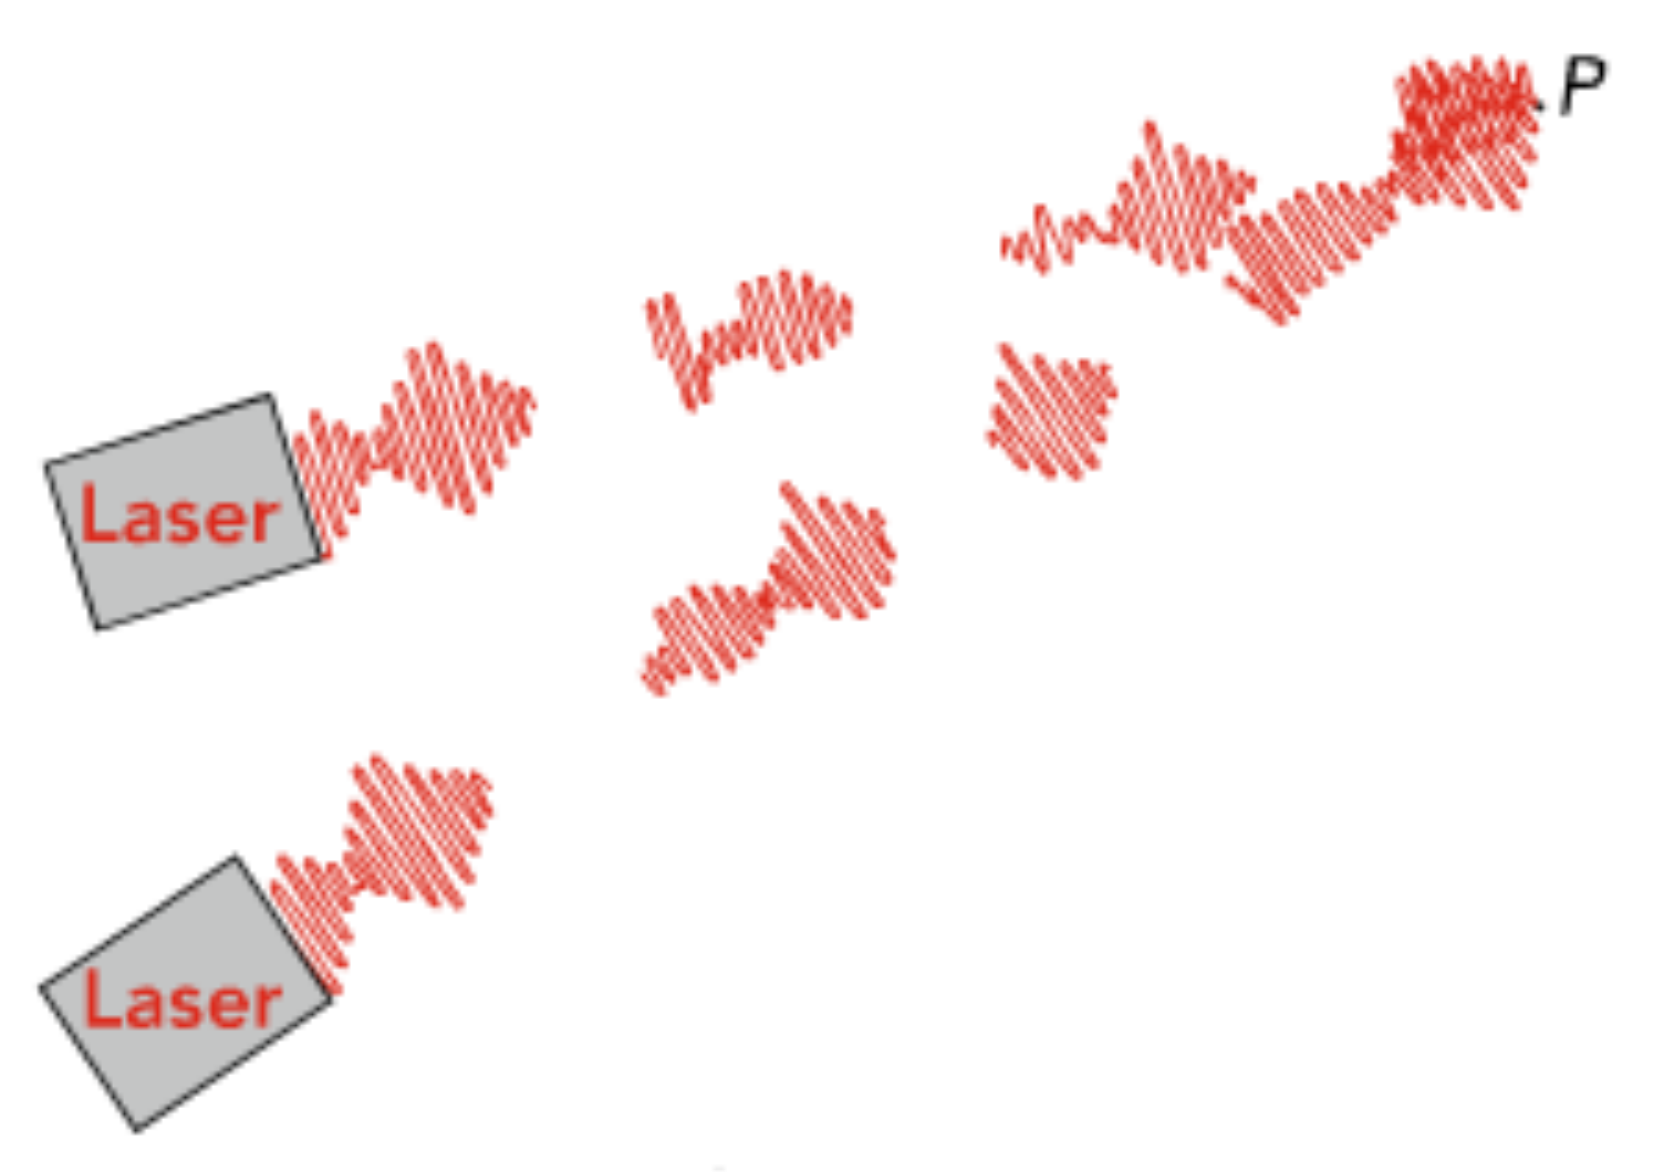
\includegraphics[width=.8\linewidth]{coherence}
	\end{center}
	\tcblower
	\begin{center}
		\captionsetup{justification=centering}
		\captionof{table}{Temps et longueurs de cohérence}
		\label{tab:tauclc}
		\begin{tabular}{lcc}
			\toprule
			Source               & $\tau_c$ (\si{s}) & $L_c$ (\si{m}) \\
			\midrule
			Lumière du Soleil    & \num{2e-15}       & \num{6e-7}     \\
			Ampoule              & \num{3e-14}       & \num{1e-5}     \\
			Raie rouge hydrogène & \num{1e-11}       & \num{4e-3}     \\
			Laser hélium-néon    & \num{1e-9}        & \num{3e-1}     \\
			\bottomrule
		\end{tabular}
	\end{center}
\end{tcb}

\subsection{Intensité lumineuse}

\begin{tcb*}[sidebyside, sidebyside align=top,
		righthand ratio=.4](prop){Intensité lumineuse}
	\tcbsubtitle{\fatbox{\textbf{En général}}}
	L'intensité lumineuse est reliée à son signal par~:
	\[\psw{\boxed{I(\Mr) = K \moy{s^2(\Mr,t)} = K s\ind{eff}{}^2}}\]
	\tcblower
	\tcbsubtitle{\fatbox{\textbf{OPPS}}}
	Pour une OPPS~:
	\[
		\psw{\boxed{I(\Mr) = \frac{1}{2}KA(\Mr)^2}}
	\]
\end{tcb*}

\begin{tcb*}(demo){Intensité lumineuse OPPS}
	La période (temporelle) typique d'une onde lumineuse est de l'ordre de
	\SI{e-15}{s}, ou $\approx \SI{1}{fs}$~: c'est une échelle de temps
	infinitésimale \textbf{bien inférieure au temps de détection} de n'importe
	quel capteur optique~: l'œil humain a un temps de réponse $\approx
		\SI{e-1}{s}$, un capteur CCD $\approx \SI{e-6}{s}$.
	\smallbreak
	Ainsi, un récepteur optique n'est sensible \textbf{qu'à l'énergie moyenne du
		signal}. Cette énergie est proportionnelle au carré de la grandeur $s(\Mr,t)$
	propagée par l'onde (ici électromagnétique), d'où l'expression précédente.
	\tcblower
	\begin{isd}[sidebyside, righthand ratio=.35]
		Pour une OPPS (monochromatique), on a donc
		\psw{%
			\[
				I(\Mr) =
				KA(\Mr)^2
				\underbracket[1pt]{\moy{\cos^2(\wt+\f(\Mr))}}_{= \frac{1}{2}} =
				\frac{1}{2}K A(\Mr)^2
			\]
		}%
		% \smallbreak
		% \vspace{-15pt}
		cohérent avec sa représentation temporelle. On le démontre aussi par
		intégration (cf.\ Ap.E6.3).
		\tcblower
		\begin{center}
			\sswitch{%
				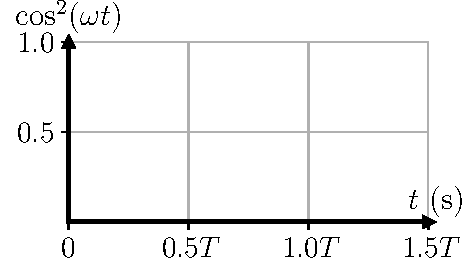
\includegraphics[width=\linewidth]{cos2_stud}
			}{%
				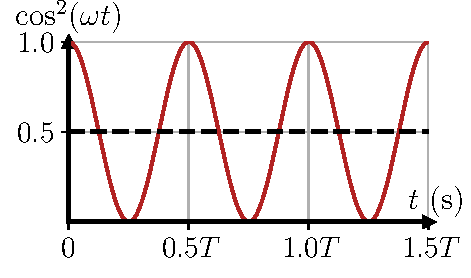
\includegraphics[width=\linewidth]{cos2_prof}
			}%
			\vspace{-15pt}
			\captionsetup{justification=centering}
			\captionof{figure}{\\$\cos^2(\wt)$ et sa moyenne.}
		\end{center}
	\end{isd}
\end{tcb*}

\subsection{Formule de \textsc{Fresnel}}
\begin{tcb}[breakable](prop){Formule de \textsc{Fresnel}}
	L'intensité lumineuse $I(\Mr)$ résultant de l'interférence de 2 ondes
	monochromatiques en un point M de l'espace s'écrit~:
	\[
		\psw{%
			\boxed{I(\Mr) = I_1 + I_2 + 2\sqrt{I_1I_2}\cos (\D\f_{2/1}(\Mr))}
		}
		\qou
		\psw{%
			\boxed{I(\Mr) = 2I_0(1+\cos (\D\f_{2/1}(\Mr)))}
		}
	\]
	si $A_1 = A_2 = A_0$, c'est-à-dire $I_1 = I_2 = I_0$. On trouve alors
	\smallbreak
	\begin{isd}[interior hidden](prop)
		\vspace{-15pt}
		\begin{gather*}
			\beforetext{\textcolor{prop}{\fatbox{\textbf{En phase}}}}
			\psw{\boxed{I\ind{max} = 4I_0}}
		\end{gather*}
		\tcblower
		\vspace{-15pt}
		\begin{gather*}
			\beforetext{\textcolor{prop}{\fatbox{\textbf{En opposition}}}}
			\hspace{40pt}
			\psw{\boxed{I\ind{min} = 0}}
		\end{gather*}
	\end{isd}
\end{tcb}

\begin{tcb}(demo)<lftt>{Formule de \textsc{Fresnel}}
	Soient 2 ondes lumineuses \textbf{cohérentes} et de même pulsation,
	d'amplitudes $A_1$ et $A_2$, interférant en un point M. On a vu que le signal
	somme $s(\Mr,t) = s_1(\Mr,t) + s_2(\Mr,t)$ avait une amplitude
	\[A(\Mr) = \sqrt{A_1{}^2 + A_2{}^2 + 2A_1A_2\cos\D\f_{2/1}(\Mr)}\]
	On trouve donc l'intensité $I(\Mr)$ en en prenant le carré et en multipliant par
	$\frac{1}{2}K$~:
	\psw{%
		\begin{gather*}
			I(\Mr)
			= \frac{1}{2}KA(\Mr)^2
			= \frac{1}{2}KA_1{}^2 + \frac{1}{2}KA_2{}^2 +
			2\frac{1}{2}KA_1A_2\cos (\D\f_{2/1}(\Mr))
			\\\beforetext{avec}
			I_1 = \frac{1}{2}KA_1{}^2
			\qet
			I_2 = \frac{1}{2}KA_2{}^2
			\qMath{on trouve}
			\sqrt{I_1I_2} = \frac{1}{2}KA_1A_2
			\qed
		\end{gather*}
	}%
	\vspace{-15pt}
\end{tcb}

\subsection{Chemin optique et déphasage}
La propagation des ondes lumineuses se fait dans des milieux avec des indices
optiques $n$ qui peuvent être différents, et donc avec des vitesses $v = c/n$
différentes. Pour continuer à travailler comme on le fait, il faut cependant que
la vitesse des signaux soient les mêmes (même fréquence et même longueur d'onde).
On définit ainsi le \textbf{chemin optique}~:
\begin{tcb*}(defi){Chemin optique}
	Le trajet d'un rayon lumineux dans un milieu d'indice $n$ entre les points A
	et B s'écrit $(\ABr)$~:
	\psw{
		\[
			\boxed{(\ABr) = n \cdot \ABr}
		\]
	}
	\vspace{-15pt}
\end{tcb*}

\begin{tcb}(demo)<lftt>{Chemin optique et $\de_{2/1}(\Mr)$}
	\psw{%
		En effet, si l'onde 1 parcourt la distance $\ABr$ dans le milieu $n$,
		elle le fait à la vitesse $v = c/n$. Pour considérer qu'elle va à la
		vitesse $c = nv$, il faut multiplier la distance par $n$~:
		\begin{gather*}
			n\ABr = nvt
			\Lra
			n\ABr = ct
		\end{gather*}
		Tout se passe comme si \textbf{l'onde allait à la vitesse $c$ mais
			parcourait une distance $n$ fois plus grande}~: on retrouve alors
		Impl.O1.2~:
		\begin{gather*}
			\boxed{\lambda = \frac{\lambda_0}{n}}
			\qqet
			-k \SaMr =
			- \frac{2\pi}{\lambda} \SaMr =
			- \frac{2\pi}{\lambda_0} \cdot n \SaMr =
			-\frac{2\pi}{\lambda_0} (\SaMr)
		\end{gather*}
	}%
	\vspace{-15pt}
\end{tcb}

\begin{tcb}(prop){Différence de chemin optique}
	Le déphasage entre 2 ondes \textit{lumineuses}, de même longueur d'onde
	$\lambda_0$ dans le vide, se superposant en M est
	\[
		\psw{%
			\boxed{\D\f_{2/1}(\Mr) = -k_0\de_{2/1}(\Mr) + \D\f_0}
		}
		\tag*{avec \psw{$k_0 = \dfrac{2\pi}{\lambda_0}$}}
	\]
	\smallbreak
	\begin{isd}[interior hidden](prop)
		\tcbsubtitle{\fatbox{\textbf{Différence de chemin}}}
		\psw{%
			\[
				\boxed{\delta_{2/1}(\Mr) = (\SbMr) - (\SaMr)}
			\]
		}%
		\vspace{-15pt}
		\tcblower
		\tcbsubtitle{\fatbox{\textbf{Déphasage à l'origine}}}
		\psw{%
			\[
				\boxed{\D\f_0 = \f_{02}-\f_{01}}
			\]
		}%
		\vspace{-15pt}
	\end{isd}
	% \begin{itemize}
	% 	\item $\de_{2/1}(\Mr) = (\SaMr) - (\SbMr)$ est la \textbf{différence de
	% 		      chemin optique} au point M.
	% 	\item $k_0 = \dfrac{2\pi}{\lambda_0}$ est le \textbf{vecteur d'onde dans
	% 		      le vide} correspondant à la \textbf{longueur d'onde dans le vide}
	% 	      des ondes.
	% 	\item $\D\f_0 = \f_{01}-\f_{02}$ est la \textbf{différence de phase à
	% 		      l'origine entre les sources}.
	% \end{itemize}
\end{tcb}

\section{Expérience des trous d'\textsc{Young}}
\subsection{Introduction}

La nature de la lumière a été sujet à de grands débats durant de nombreux
siècles, entre vision corpusculaire et ondulatoire. C'est en 1802 que
l'expérience dite des «~trous d'\textsc{Young}~» a permis de confirmer la nature
ondulatoire de la lumière en réalisant une figure d'interférences
lumineuses\ftn{Voir la vidéo \href{https://youtu.be/zPolTp0ddRg}{La plus belle
		expérience de la Physique}}. Une version moderne de cette expérience
consiste à pointer un unique laser de longueur d'onde $\lambda_0$ sur deux fentes
fines horizontales et parallèles~: ces fentes diffractent la lumière est se
comportent \textbf{comme deux sources cohérentes}.

% \bigbreak
% En effet, pour obtenir 2 sources lumineuses cohérentes il faut créer deux
% sources secondaires provenant d'une \textbf{source unique} et qui ait un temps
% de cohérence suffisamment grand. Une version moderne de cette expérience
% consiste à pointer un unique laser de longueur d'onde $\lambda$ sur deux fentes
% fines horizontales et parallèles~: ces fentes diffractent la lumière est se
% comportent \textbf{comme deux sources cohérentes}.

\begin{tcb}(defi){Description du résultat}
	\begin{isd}
		La zone de l'espace où les faisceaux se superposent est appelé \textbf{champ
			d'interférences}. Sur un écran, on observe alors des variations
		d'intensité lumineuse~:
		\begin{itemize}
			\item au milieu des zones claires (\textbf{maximum} local d'intensité)
			      on a des \textbf{interférences constructives}~;
			\item au milieu des zones sombres (\textbf{minimum} local d'intensité)
			      on a des \textbf{interférences destructives}.
		\end{itemize}
		\tcblower
		\begin{center}
			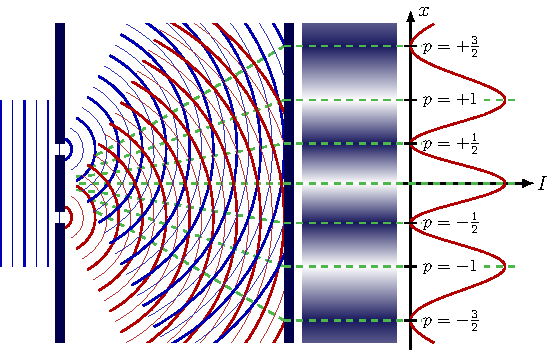
\includegraphics[width=\linewidth]{young_result}
			\captionof{figure}{Figure d'interférence.}
		\end{center}
	\end{isd}
	On appelle \textbf{interfrange} et on le note $i$ la \textbf{distance}
	séparant \textbf{deux milieux de franges} brillantes (ou sombres)
	consécutives.
\end{tcb}

\subsection{Présentation}

\begin{tcb*}[breakable](defi){Présentation trous d'\textsc{Young}}
	Soit S une source lumineuse ponctuelle, monochromatique de longueur d'onde
	$\lambda_0$, éclairant deux fentes fines horizontales et parallèles F$_1$ et
	F$_2$ distantes de $2a$, avec O au milieu. S est situé sur un axe optique
	perpendiculaire à un écran placé à une distance $D$ très supérieure à $a$
	(pour l'approximation en ondes planes). Le milieu de propagation est l'air,
	d'indice optique $n=1$.
	\begin{center}
		\sswitch{
			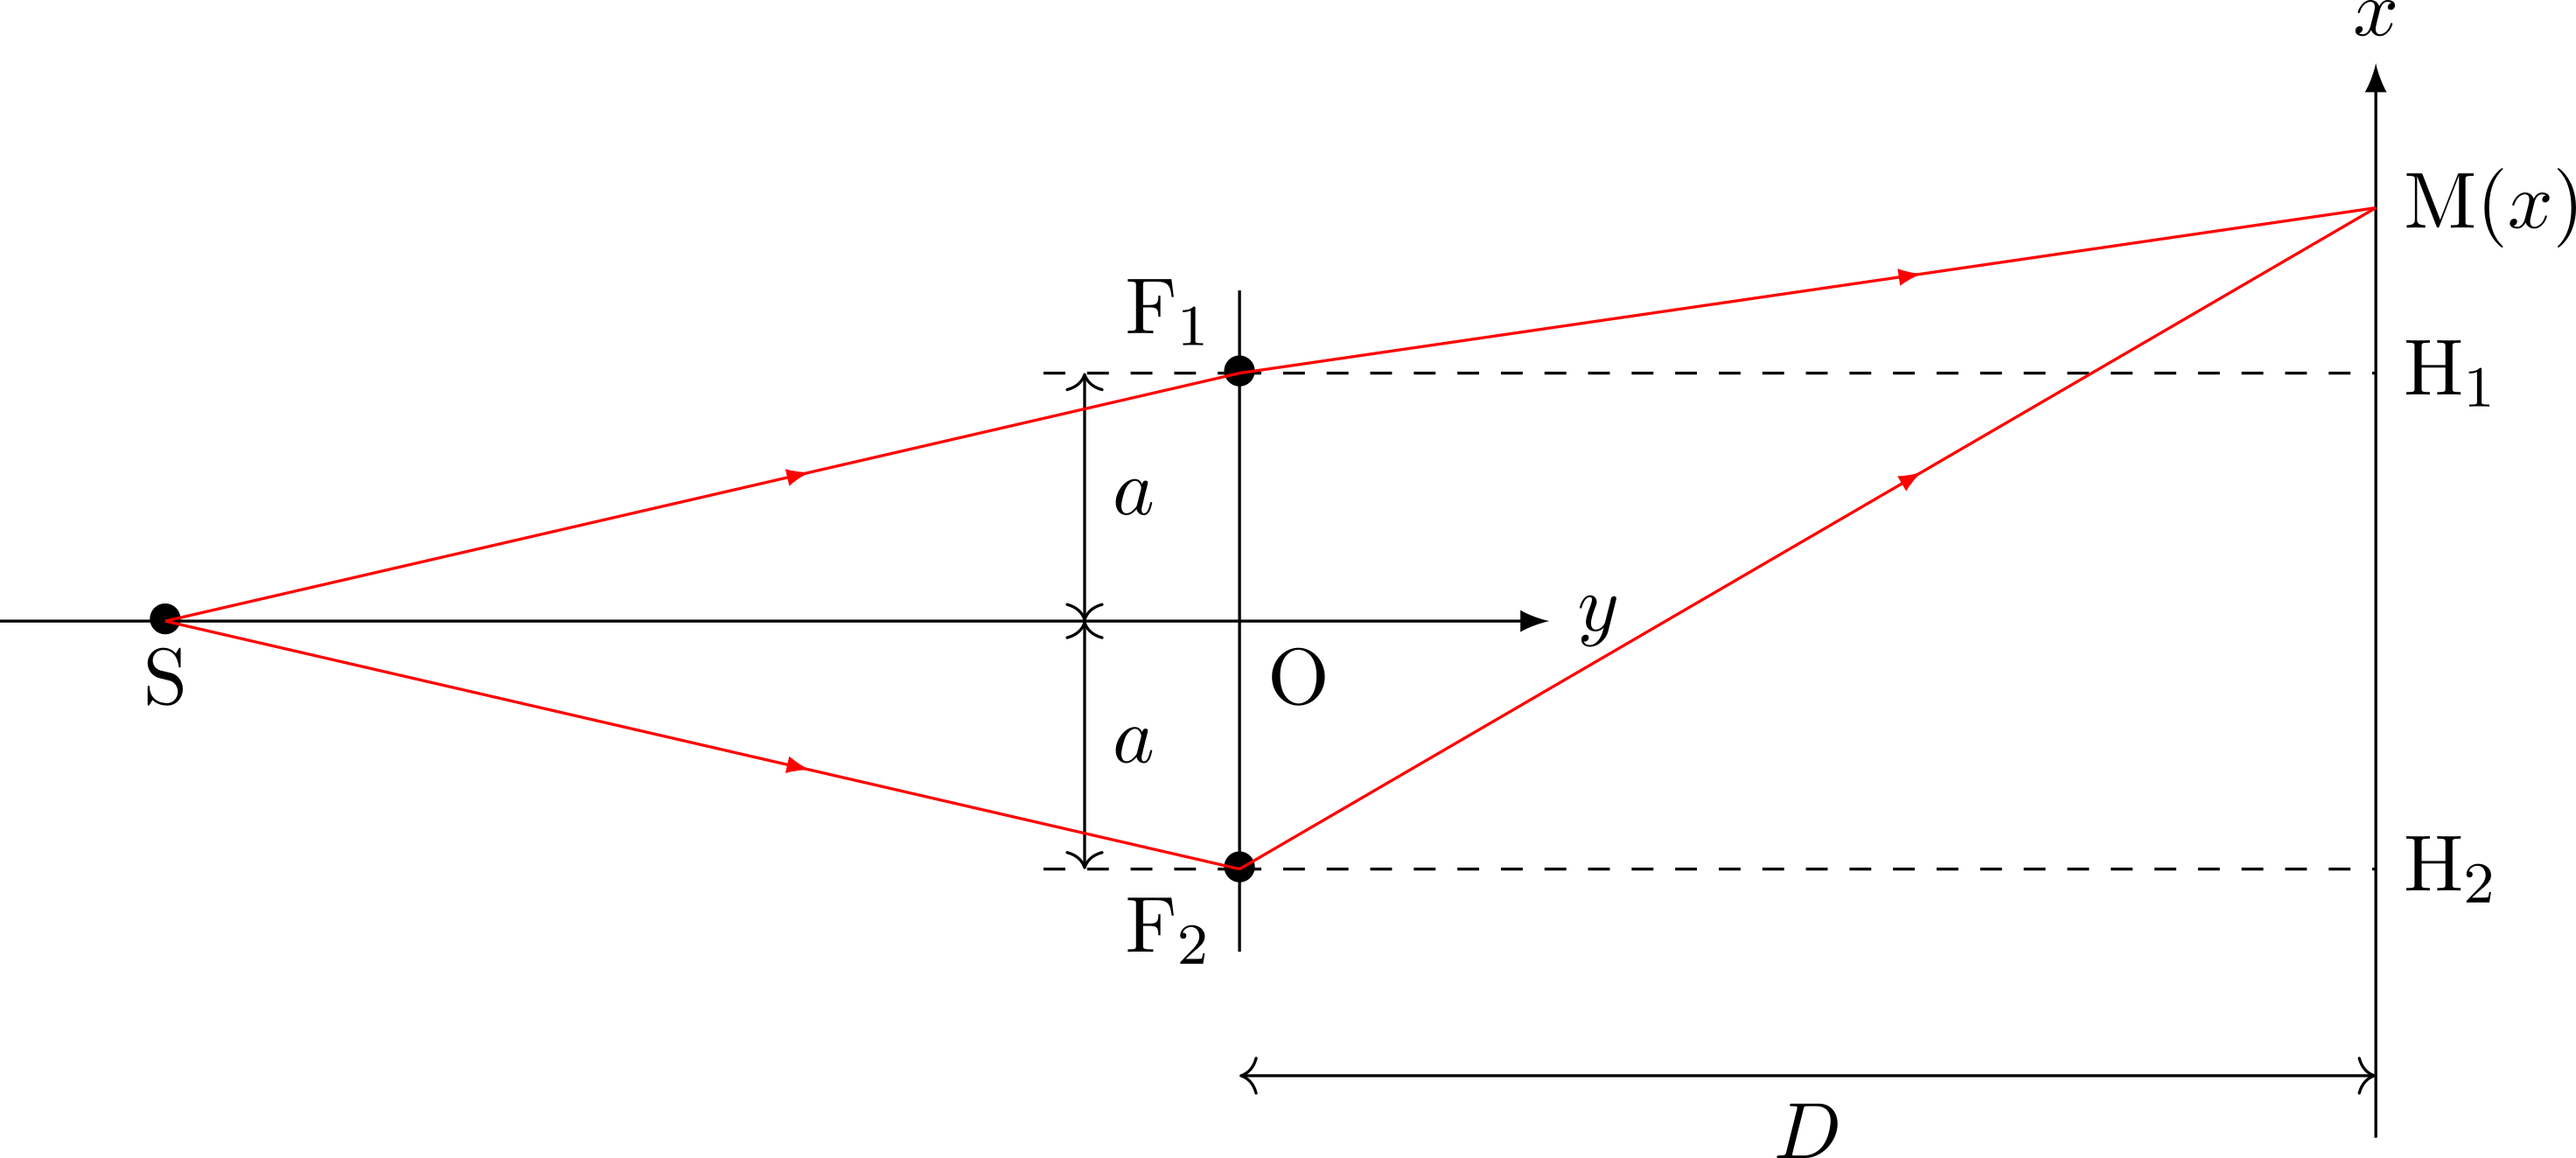
\includegraphics[width=.7\linewidth, draft=true]{yhole}
		}{
			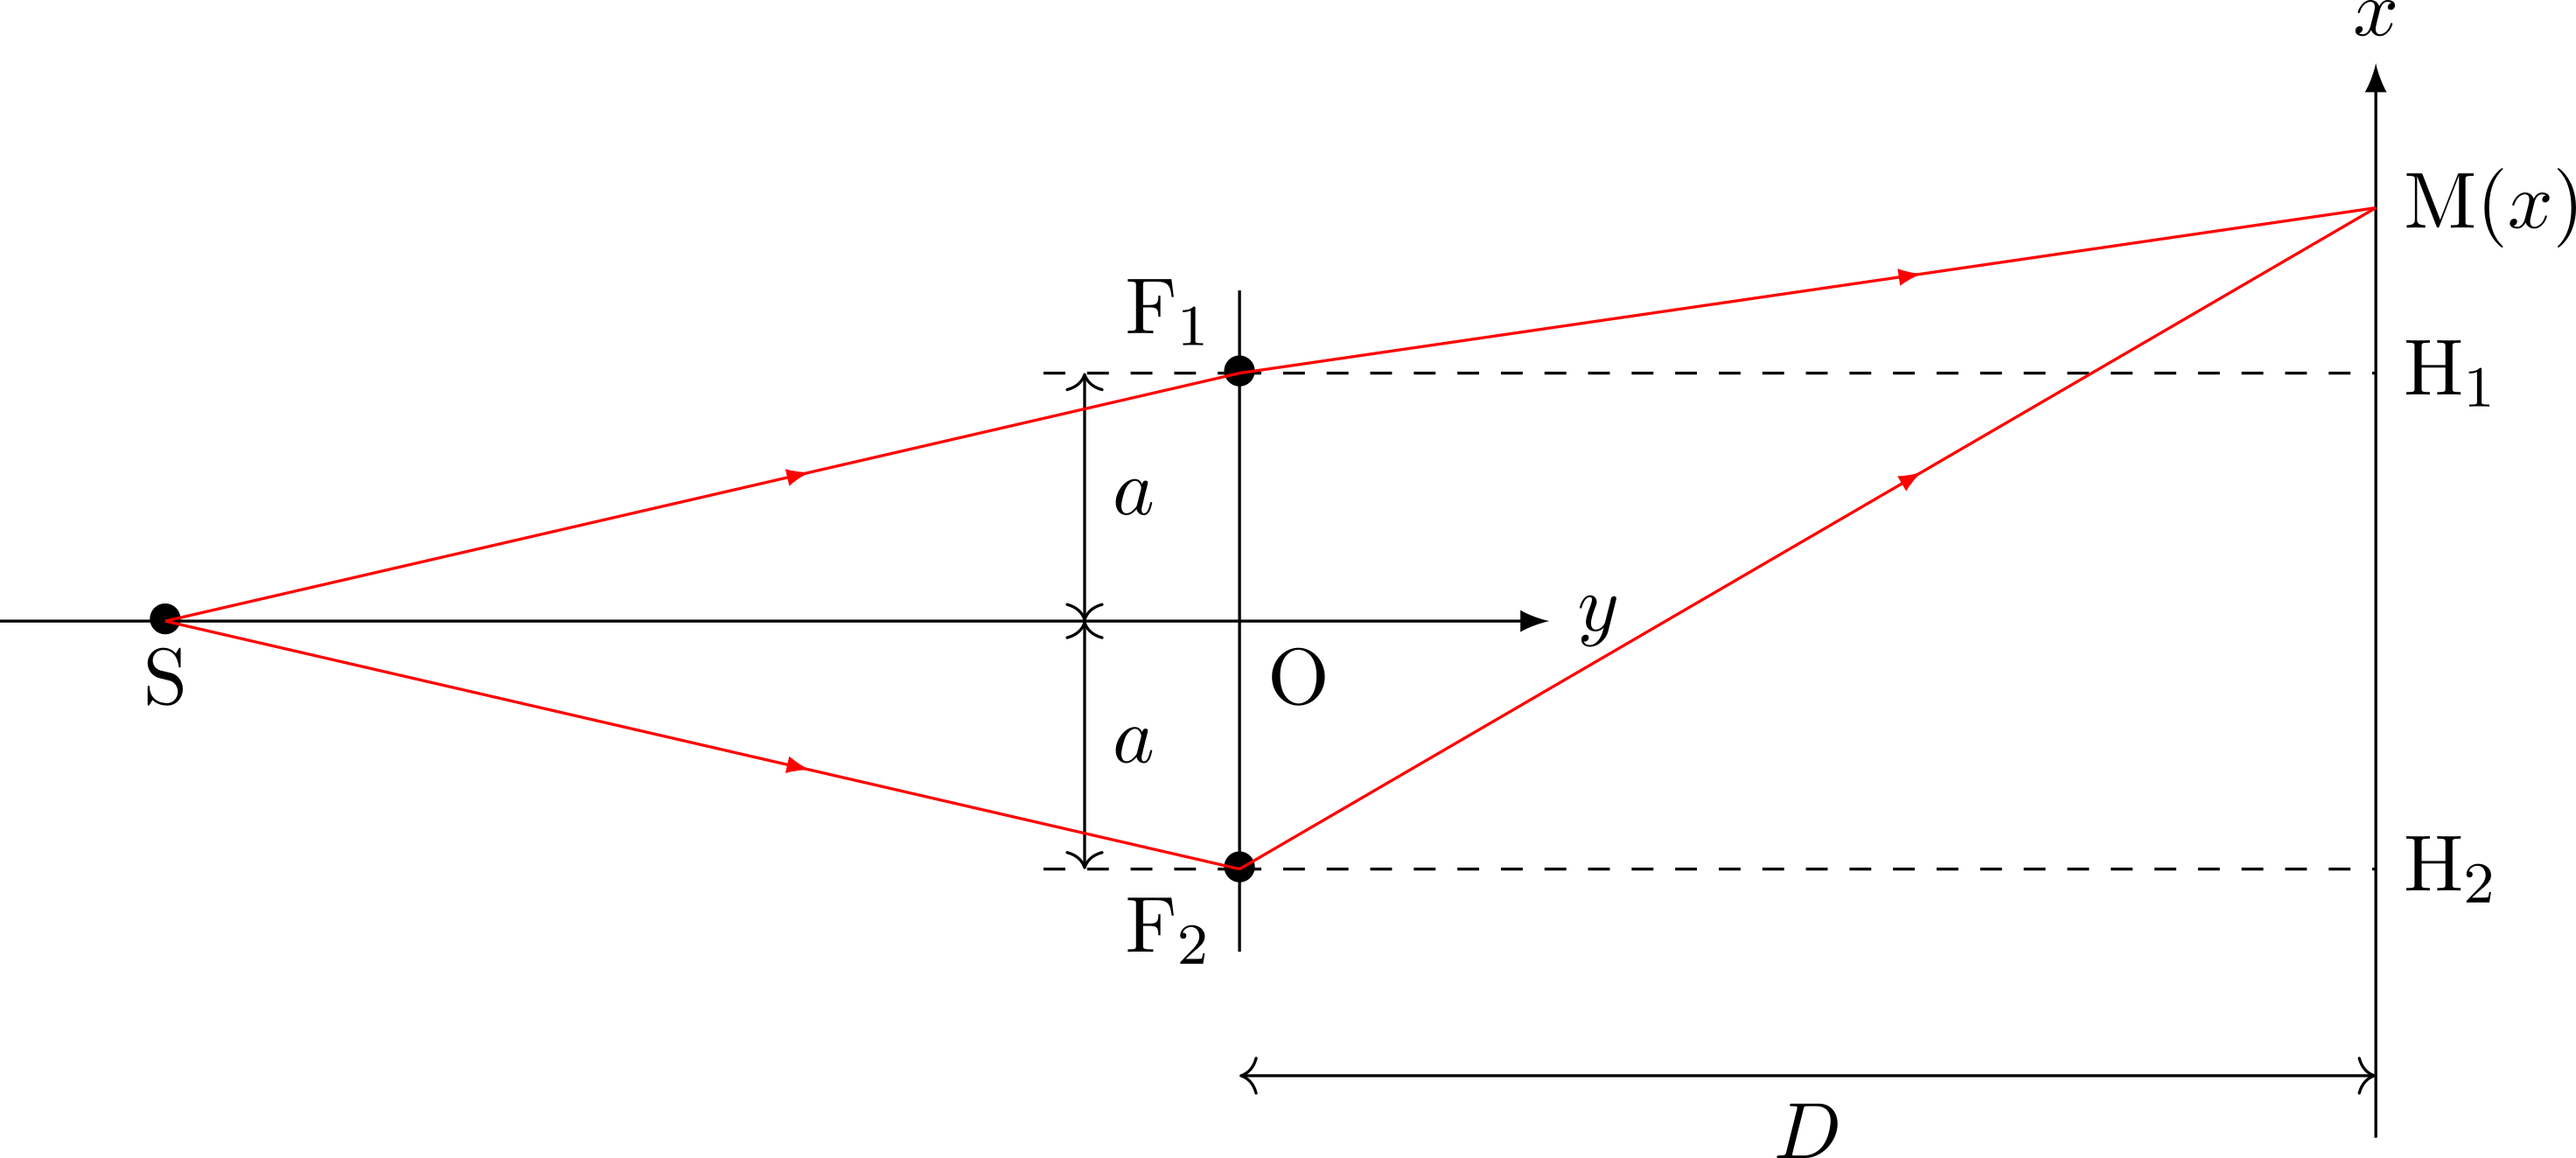
\includegraphics[width=.7\linewidth]{yhole}
		}
		\captionof{figure}{Schéma des trous d'\textsc{Young}}
		\label{fig:yhole}
	\end{center}
\end{tcb*}
On se limite au tracé de 2 rayons qui interfèrent au point M$(x)$, passant
chacun par une des fentes (voir Figure~\ref{fig:yhole}). On a alors
successivement~:

\begin{tcb*}(inte)<lftt>{Expérience des trous d'\textsc{Young}}
	\begin{itemize}
		\item[b]{Diffraction}~:
		      \psw{%
			      quand l'\textbf{ouverture est de l'ordre de la longueur d'onde}, on
			      observe un étalement du faisceau. Chaque trou créé une
			      \textbf{tâche de diffraction}, et ces deux tâches \textbf{se
				      superposent sur l'écran} en créant des interférences observables.
		      }%
		\item[b]{Interférences}~:
		      avec la formule de \textsc{Fresnel} pour des intensités égales,
		      \[
			      I(\Mr) = 2I_0 \pa{1+\cos(\Delta{\f}_{2/1}(\Mr))}
		      \]
		      \begin{itemize}
			      \item[b]{Constructives}~:
			            \psw{%
				            pour $\D\f_{2/1}(\Mr) = 2p\pi \Lra \boxed{\delta_{2/1}(\Mr)
						            = p\lambda_0}$~;
			            }%
			      \item[b]{Destructives}~:
			            \psw{%
				            pour $\D\f_{2/1}(\Mr) = (2p+1)\pi \Lra
					            \boxed{\delta_{2/1}(\Mr) = (2p+1)\frac{\lambda_0}{2}}$.
			            }%
		      \end{itemize}
	\end{itemize}
	\vspace{-15pt}
\end{tcb*}

% On va donc déterminer le déphasage puis la différence de chemin de ces rayons,
% pour finalement déterminer l'interfrange $i$.

\subsection{Résolution}
\begin{tcb*}[sidebyside, righthand ratio=.5](prop){Intensité et interfrange}
	Pour $I_1 = I_2 = I_0$, on obtient
	\[
		\psw{%
			\boxed{I(\Mr) = 2I_0 \left( 1 + \cos (\frac{4\pi ax}{\lambda_0 D}) \right)}
		}
	\]
	décrivant des franges, espacées de
	\[
		\psw{%
			\boxed{i = \frac{\lambda_0 D}{2a}}
		}
	\]
	\tcblower
	\begin{center}
		
\includegraphics[width=\linewidth]{young_intensity}
		\captionof{figure}{Franges avec atténuation.}
	\end{center}
\end{tcb*}

\begin{tcb*}[breakable](demo){Intensité et interfrange}
	\tcbsubtitle{\fatbox{\textbf{Intensité}}}
	\vspace{-15pt}
	\psw{%
		\begin{gather*}
			\delta_{2/1}(\Mr) =
			(\SMr)_2 - (\SMr)_1 =
			\rm \cancel{\rm SF_2} + F_2M - (\cancel{\rm SF_1} + F_1M)
			\\\Lra
			\boxed{\delta_{2/1}(\Mr) = \rm F_2M - F_1M}
		\end{gather*}
	}%
	On cherche donc à exprimer $\rm F_1M$ et $\rm F_2M$. Pour cela, on place les
	points H$_1$ et H$_2$ projetés orthogonaux de F$_1$ et F$_2$ sur l'écran,
	créant ainsi deux triangles rectangles~: $\rm F_1H_1M$ et $\rm F_2H_2M$.
	\begin{align*}
		\psw{{\rm F_2M^2 = F_2H_2{}^2 + H_2M^2}}
		 & \qet
		\psw{{\rm F_1M^2 = F_1H_1{}^2 + H_1M^2}}
		\\
		\psw{\Lra{\rm F_2M} = \sqrt{D^2 + (x+a)^2}}
		 & \qet
		\psw{{\rm F_1M} = \sqrt{D^2 + (x-a)^2}}
		\\
		\psw{\Lra{\rm F_2M} = D \sqrt{1+ \left( \frac{x+a}{D} \right)^2}}
		 & \qet
		\psw{{\rm F_1M} = D \sqrt{1+ \left( \frac{x-a}{D} \right)^2}}
		\intertext{Or, $\DS\sqrt{1+\ep} \Sim_{\ep \to 0} 1 + \frac{\ep}{2}$~; comme
			$\DS D \gg (x~;~a) \Ra \frac{x\pm a}{D} \ll 1$, alors avec $\DS \ep =
				\pa{\frac{x \pm a}{D}}^2$ on a~:}
		\psw{%
			{\rm F_2M} \approx D \pa{1 + \frac{1}{2} \left( \frac{x+a}{D} \right)^2}
		}%
		 & \qet
		\psw{%
			{\rm F_1M} \approx D \pa{1 + \frac{1}{2} \left( \frac{x-a}{D} \right)^2}
		}%
		\\
		\psw{\Lra{\rm F_1M} = D + \frac{(x-a)^2}{2D}}
		 & \qet
		\psw{{\rm F_2M} = D + \frac{(x+a)^2}{2D}}
	\end{align*}
	\vspace{-15pt}
	\psw{%
		\begin{align*}
			\beforetext{\blk{Ainsi,}}
			{\rm F_2M - F_1M} & = \frac{(x+a)^2 - (x-a)^2}{2D}
			\tag*{}
			\\ \Lra
			\de_{2/1}(\Mr)    & = \frac{(x+\cancel{a}+x-\cancel{a})
				\times(\bcancel{x}+a-(\bcancel{x}-a))}{2D}
			\\ \Lra
			\de_{2/1}(\Mr)    & = \frac{4ax}{2D}
			\Lra
			\boxed{\de_{2/1}(\Mr) = \frac{2ax}{D}}
			\\\beforetext{\blk{Soit}}
			I(\Mr)            & =
			2I_0 \pa{1+ \cos(-\frac{2\pi}{\lambda_0} \frac{2ax}{D})}
			\\\Lra
			\Aboxed{I(\Mr)    & = 2I_0 \pa{1+ \cos(\frac{4\pi ax}{\lambda_0 D})}}
			\qed
		\end{align*}
	}%
	\vspace{-15pt}
	\tcbsubtitle{\fatbox{\textbf{Interfrange}}}
	\begin{itemize}
		\item[b]{Interférences constructives}~:
		      \vspace{-15pt}
		      \psw{%
			      \begin{gather*}
				      \delta_{2/1}(\Mr) = p\lambda_0
				      \Lra
				      \boxed{x_p = p \frac{\lambda_0 D}{2a}}
				      \tag*{$p \in \Zb$}
			      \end{gather*}
		      }%
		      \vspace{-15pt}
		\item[b]{Interférences destructives}~:
		      \vspace{-15pt}
		      \psw{%
			      \begin{gather*}
				      \delta_{2/1}(\Mr) = \pa{2p + 1} \frac{\lambda_0}{2}
				      \Lra
				      \boxed{x'_p = \pa{p + \frac{1}{2}} \frac{\lambda_0D}{2a}}
				      \tag*{$p \in \Zb$}
			      \end{gather*}
		      }%
		      \vspace{-15pt}
		\item[b]{Interfrange}~:
		      \vspace{-15pt}
		      \psw{%
			      \begin{gather*}
				      i = x_{p+1} - x_p
				      \Lra
				      \boxed{i = \frac{\lambda_0 D}{2a}}
				      \qed
			      \end{gather*}
		      }%
	\end{itemize}
	\vspace*{-15pt}
\end{tcb*}

\begin{tcb}(exem)<lftt>{Interfrange}
	Avec deux fentes séparées de \SI{0.20}{mm}, $\lambda_0 = \SI{632}{nm}$ et $D =
		\SI{1.0}{m}$, on trouve\ftn{Voir une autre animation \href{https://phyanim.sciences.univ-nantes.fr/Ondes/lumiere/interference_lumiere.php}{ici}.}
	\psw{%
		\[\xul{i = \SI{1.6}{mm}}\]
	}%
	\vspace{-25pt}
\end{tcb}

\end{document}
